\documentclass[12pt]{article}
\usepackage[tables,figures,master]{updiplom}
\usepackage[utf8]{inputenc}
\usepackage{amsmath}
\usepackage{amsthm}
\usepackage{booktabs}
\usepackage{algorithm}
\usepackage{algpseudocode}
\usepackage{url}

\DeclareUrlCommand\url{\def\UrlLeft{<}\def\UrlRight{>} \urlstyle{tt}}


%%% Obecné věci
\newcommand{\name}{CLaSeek}
\newcommand{\nameurl}{\url{http://phoebe.inf.upol.cz/fcasearch/}}
\newcommand{\code}[1]{\texttt{#1}}
\newcommand{\sep}{\,|\,}
\newcommand{\docs}{\mathbb{D}}
\newcommand{\yes}{$\times$}
\newcommand{\fyes}{\fbox{$\times$}}
\newcommand{\foreach}{\mbox{pro všechna }}
\newcommand{\pravekdyz}{\mbox{právě když }}

%%% Nadpisy
\newcommand{\ssection}[1]{\subsection{#1}}
\newcommand{\sssection}[1]{\subsubsection{#1}}

%%% Závorky
\newcommand{\addk}[1]{\left(#1\right)}
\newcommand{\addh}[1]{\left[#1\right]}
\newcommand{\adds}[1]{\left\{#1\right\}}
\newcommand{\addsp}[1]{\left<#1\right>}

\newcommand{\strong}[1]{{\em #1}}

%%% Logické spojky
\newcommand{\logand}{\,\wedge\,}
\newcommand{\logor}{\,\vee\,}
\newcommand{\eq}{\Leftrightarrow}
\renewcommand{\implies}{\Rightarrow}

%%% Používané funkce
\DeclareMathOperator{\fix}{fix}
\DeclareMathOperator{\tfidf}{tf-idf}
\DeclareMathOperator{\stem}{stem}
\DeclareMathOperator{\score}{sc}
\DeclareMathOperator{\wcount}{sf}
\DeclareMathOperator{\getdocs}{R}
\DeclareMathOperator{\AND}{AND}
\DeclareMathOperator{\OR}{OR}
\DeclareMathOperator{\NOT}{NOT}
\DeclareMathOperator{\rank}{rank}
\DeclareMathOperator{\ext}{Ext}
\DeclareMathOperator{\intfca}{Int}
\DeclareMathOperator{\lowerneighbors}{LowerNeighbors}
\DeclareMathOperator{\upperneighbors}{UpperNeighbors}
\DeclareMathOperator{\unfca}{UN}
\DeclareMathOperator{\lnfca}{LN}
\DeclareMathOperator{\simfca}{sim}

\newcommand{\invstem}{\stem^{-1}}
\newcommand{\alldoc}{\mathbb{D}}

%%% FCA věci
\newcommand{\context}{\addsp{X, Y, I}}
\newcommand{\lattice}{\mathcal{B}(X, Y, I)}
\newcommand{\AB}{\addsp{A, B}}
\newcommand{\up}{^{\uparrow}}
\newcommand{\down}{^{\downarrow}}
\newcommand{\updown}{^{\uparrow\downarrow}}
\newcommand{\downup}{^{\downarrow\uparrow}}
\newcommand{\biginf}{\bigwedge}
\newcommand{\bigsup}{\bigvee}
\newcommand{\hledany}{\mathbb{H}}
\newcommand{\lowerc}{\mathbb{L}}
\newcommand{\upperc}{\mathbb{U}}
\newcommand{\sibl}{\mathbb{S}}



\newtheorem{mydef}{Definice}
\newtheorem{theorem}[mydef]{Věta}

\clubpenalty 10000
\widowpenalty 10000



\title{Vyhledávač založený na formální konceptuální analýze}
\author{Lukáš Havrlant}
\year{2011}
%\date{21. květen 2009}

\docinfo{Lukáš Havrlant}{Vyhledávač založený na formální konceptuální analýze}

\annotation{Napovídáním souvisejících dotazů může vyhledávač pomoci uživateli rychleji najít dokumenty, které potřebuje. Práce se zabývá tvorbou vyhledávače s webovým rozhraním, který pracuje nad uzavřenou sadou dokumentů. Po položení dotazu dokáže napovědět konkrétnější, obecnější a podobný dotaz, což je realizováno pomocí formální konceptuální analýzy.}

\thanks{Děkuji Mgr. Janu Outratovi, Ph.D. za vedení této diplomové práce a za rady při konzultacích.}

\begin{document}

\maketitle
\newpage


%%% Text diplomové práce.
\section*{Úvod}
\addcontentsline{toc}{section}{Úvod}

Současné vyhledávače si uchovávají obsah, nad kterým mají vyhledávat, ve formě indexu, což je struktura v principu podobná indexu v knize. Uživateli stačí vložit do vyhledávacího pole svůj dotaz a vyhledávač z indexu získá potřebná data a zobrazí uživateli výsledek, obvykle ve formě nějakého uspořádaného seznamu odkazů na dokumenty. Pokud není uživatel spokojený s výsledky, musí přeformulovat svůj dotaz tak, aby lépe vystihoval to, co chce najít. 

Tento problém je typický pro slova, která mají několik významů. Například pokud ve webovém vyhledávači vyhledáme slovo \uv{jaguár}, tak vyhledávač nemůže vědět, zda chceme hledat auto, zvíře nebo ještě něco jiného. Pokud má přístup k historii hledání daného uživatele, může pomocí ní přizpůsobit výsledky. Ale může také uživateli zobrazit návrhy na nový dotaz, například \uv{jaguár auto} nebo \uv{jaguár zvíře}, po jejichž vyhledání se výsledky velmi zpřesní. 

Otázkou je, jak tyto návrhy získat. Pokud si vyhledávač uchovává historii všech hledání, která uživatelé provádějí, může se je pokusit vytáhnout právě z této historie. Pokud ovšem tato data vyhledávač nemá, nebo jich má málo, musí se použít jiná metoda. 

Práce popisuje metodu, jak získat podobné dotazy pomocí formální konceptuální analýzy (anglicky Formal concept analysis, dále jen FCA) pouze na základně znalosti obsahu dokumentů. FCA pracuje s tabulkovými daty, ve kterých hledá nějaké potenciálně zajímavé shluky dat. Tyto shluky pro nás budou představovat množiny dokumentů, které jsou nějakým způsobem podobné a které sdílí nějaká zásadní klíčová slova. Tato klíčová slova poté dále využijeme při generování návrhů na nové dotazy. 

\newpage
\section{Information retrieval}

Tato sekce se zabývá budováním samotného vyhledávače, jehož výsledky budou zobrazeny uživateli a také budou použity jako vstup do formální konceptuální analýzy. 

Cílem je popsat tvorbu vyhledávače, který bude umět stáhnout z webu požadované dokumenty, zaindexovat je a následně v nich vyhledávat. Dokumenty mohou být buď obyčejné webové stránky nebo složitější soubory, například PDF. 

\subsection{Jak funguje vyhledávač}
V této části si popíšeme, jak může obecný vyhledávač fungovat. 

\subsubsection{Pojmy související s vyhledávačem}
\begin{description}
\item[Sada dokumentů] Na začátku máme nějakou sadu dokumentů, nad kterými chceme vyhledávat. Tato sada může být libovolná -- může se jednat o webové stránky, o lokální dokumenty na osobním počítači nebo o emaily na serveru. V případě webových vyhledávačů typu Google je pak sadou dokumentů \uv{všechno, co lze nalézt na webu}, v případě vyhledávačů v moderních operačních systémech je sadou \uv{všechno, co lze nalézt na počítači}. 

Sada dokumentů může být statická, nebo dynamická. Statická sada je taková sada, která se nemění buď nikdy nebo málokdy. Může to být například vyhledávač PSČ. Dynamická sada se naopak mění poměrně často, například webové stránky. Velké vyhledávače častěji pracují s dynamickou sadou dokumentů. 

\item[Uživatel] Uživatel je obecné označení toho, kdo pracuje s vyhledávačem. Typicky se jedná o nějakého člověka, ale může to být i program, který například každý den kontroluje počet dokumentů na dané klíčové slovo a při zvýšení tohoto počtu pošle někomu informační email. 

\item[Dotaz] Pomocí dotazů komunikuje uživatel s vyhledávačem. Dotaz je nějaký seznam slov, který reprezentuje to, co uživatel chce najít. Může se jednat o jednoduché dotazy typu \uv{auto}, ale také o složitější otázky jako \uv{Jaký je smysl života?} Slovům v dotazu říkáme klíčová slova. 

Vyhledávač může uživatelům umožnit používat v dotazu různé operátory, kterými lze zpřesnit dotaz. Typické operátory jsou logické operátory AND, OR a NOT. Webové vyhledávače umožňují například vyhledávat na určité doméně pomocí SITE operátoru, vyhledat odkazující stránky pomocí LINK operátoru a podobně. 

\item[Výsledky vyhledávání] Po položení dotazu zobrazí vyhledávač výsledky. Obecně se jedná o nějaké zkrácené zobrazení dokumentů, které vyhovují danému dotazu. Typicky jde o seznam odkazů na dané dokumenty, ale v některých případech může vyhledávač přímo zodpovědět položenou otázku. Například na otázku o smyslu života může odpověď 42. 

Samotný seznam dokumentů bývá obvykle seřazen podle nějakých kritérií. Těchto kritérií bývá poměrně hodně a vyvážit je tak, aby vyhledávač vracel co možná nejlepší výsledky je obtížný úkol, kterým se tato diplomová práce nebude více zabývat. 

Mezi výsledky může být kromě seznamu odkazů i nějaká další informace. Současné webové vyhledávače například umí opravovat překlepy, přehrát video odpovídající klíčovým slovům, vypočítat jednoduché matematické operace nebo napovědět dotaz, který by vedl k přesnějším výsledkům. 
\end{description}


Dále si představíme dva modely, jak může vyhledávač fungovat. Naivní model a model používající index.

\subsubsection{Naivní model vyhledávače}

Naivní model vyhledávače funguje tak, že po položení dotazu začne vyhledávač procházet všechny dokumenty a kontroluje, jestli některý z dokumentů odpovídá dotazu. Pokud ano, vrátí tento dokument mezi výsledky. 

Tento model je velice jednoduchý, ale není příliš efektivní. V současné době můžeme mít sady dokumentů, které obsahují miliony či miliardy položek, takže chceme-li znát výsledky řádově za desetiny sekund, není možné je při každém dotazu všechny procházet.

\subsubsection{Vyhledávač používající index}
Mnohem efektivnější je použít index. Jedná se o podobnou strukturu, kterou můžeme najít v některých, obzvláště odborných, knihách. Protože v klasické tištěné knize nemůžeme nijak \uv{vyhledávat}, dává se na konec knihy seznam nejdůležitějších slov, která kniha obsahuje, spolu s čísly stránek, na kterých se pojem vyskytuje. Takže chce-li uživatel nalézt stránky obsahující slovo \uv{derivace}, podívá se do indexu, kde hned zjistí, že slovo se vyskytuje na té a té stránce. 

Podobný princip můžeme použít i ve vyhledávačích. Nebudeme ale vytvářet index z důležitých slov, ale ze všech slov, která se v dokumentech vyskytují. Vytvoříme tak slovníkovou strukturu, kde klíčem bude slovo a hodnotou bude seznam dokumentů, které dané slovo obsahují. Při položení dotazu pak může vyhledávač rychle zjistit jaké dokumenty obsahují dané klíčové slovo prostým nahlédnutím do tohoto slovníku. 

Spolu s tím si můžeme uložit informace i o tom, kolik daných slov daný dokument obsahuje, což můžeme dále využít při řazení dokumentů. 

Celou práci vyhledávače tak můžeme rozdělit do dvou částí -- budování a upravování indexu a hledání odpovědí na dotaz. Zde je nutné dát pozor na to, jak velká je sada dokumentů a zda je statická nebo dynamická. Samotné budování indexu můžeme ještě rozdělit na dvě části: předzpracování dokumentů a technická realizace indexu. 

\subsection{Vyhledávač \name}

Součástí této diplomové práce je naprogramovaný vyhledávač \name{} (Concept Lattice Seeker), který bude v dalších částech textu popsán. \name{} je vyhledávač napsaný v Pythonu 3. Pracuje se statickou sadou dokumentů; předpokládá se, že se sada dokumentů bude měnit pouze nárazově jednou za čas. Samotná sada dokumentů, nad kterou má vyhledávač pracovat, nebude příliš velká, řádově stovky dokumentů. 

Jedná se o vyhledávač používající index. Při budování indexu je vstupem seznam URL adres, který si vyhledávač sám stáhne a zaindexuje obsahy dokumentů. Výsledný index je pak uložen do několika souborů, ke kterým pak \name{} přistupuje. 

\name{} má rozumět logickým operátorům AND, OR a NOT. Po zadání dotazu má vrátit výsledky seřazené podle relevance, kterou spočítá pomocí klasického $\tfidf$ algoritmu. Výstup bude textový ve formátu JSON, se kterým pak mohou pracovat další programy, v tomto případě webové rozhraní, které je napsáno v PHP. 

Další částí vyhledávače je hledání souvisejících dotazů. Tato část bude podrobně rozebrána v další kapitole. V této kapitole je dále popsáno, jak \name{} buduje index a jak vrací výsledky. 

%Dále seznam dotazů, které konkretizují zadaný dotaz, tj. seznam nových klíčových slov, které můžeme přidat k současnému dotazu, abychom získali přesnější výsledky. To je případ, kdy po vyhledání \uv{jaguár} vyhledávač napoví \uv{jaguár auto}. Dále seznam podobných dotazů, což jsou dotazy, které mění jedno nebo více klíčových slov v dotazu. To je případ, kdy vyhledávač k \uv{jaguár auto} napoví \uv{jaguár zvíře}. Nakonec vyhledávač zobrazí i obecnější dotaz. K dotazu \uv{jaguár zvíře} tak může zobrazit \uv{jaguár}.  


\subsection{Předzpracování dokumentů}
\label{prepr}
Při budování indexu máme na vstupu sadu dokumentů a na výstupu strukturu, která reprezentuje index této sady. Během samotného budování indexu procházíme jednotlivé dokumenty a upravujeme je do takové podoby, která se hodí pro uložení. Budeme uvažovat pouze textové dokumenty jako je HTML nebo PDF a budeme předpokládat statickou sadu dokumentů, takže se nebudeme příliš zatěžovat aktualizací indexu. 

Na samotném začátku tak musíme upravit jednotlivé textové dokumenty do nějaké kanonické podoby. To budeme dělat postupnými úpravami jednotlivých dokumentů. S každým dokumentem budeme provádět identické operace v identickém pořadí. Jednotlivé operace budou popsány v takovém pořadí, v jakém se aplikují ve vyhledávači. Všechny operace jsou popsány v knihách \cite{modernir}, kapitola 7 a \cite{introir}, kapitola 2.

\begin{description}
% \item[Zjištění názvu dokumentu] U některých typů dokumentů můžeme z jejich obsahu zjistit název dokumentu. Například pokud máme na vstupu HTML stránku, můžeme zjistit název stránky z TITLE elementu. U ostatních dokumentů vezmeme jako název obyčejný název souboru. Pokud zpracováváme soubor \code{prikazy.pdf}, bude názvem právě \uv{prikazy.pdf}.

\item[Odstranění formátovacích prvků dokumentu] Vstupem do algoritmu budování indexu může být soubor, který kromě samotného textu obsahuje i různé formátovací a jiné prvky. Tyto prvky pro další zpracování nepotřebujeme, takže je všechny odstraníme. Jedná se například o HTML nebo XML značky. Po aplikaci tohoto bodu už bychom měli mít pouze čistý text. 

\item[Ponechání písmen] Text obsahuje spousty různých znaků, které jsou vyhledávači téměř k ničemu. Jedná se o interpunkci, která typicky doplňuje text, ale při samotném vyhledávání se bez ní obejdeme. Odstraníme tak všechny znaky, které nejsou písmeny. 

Při tomto odstraňování můžeme narazit na určité problémy a může zde dojít k první ztrátě informace. Například pokud ze slova \uv{chcete-li} odstraníme spojovník, můžeme dostat buď slovo \uv{chceteli} nebo dvě slova \uv{chcete} a \uv{li}. 

\item[Odstranění bílých znaků] Pod bílé znaky spadají mezery, tabulátory a nové řádky. To jsou opět informace, které jsou zbytné a které můžeme odstranit. Namísto libovolně dlouhé posloupnosti bílých znaků tak vždy vložíme právě jednu mezeru. Tím dosáhneme toho, že všechna slova v celém dokumentu budou v jednom řádku a budou oddělena právě jednou mezerou. 

\item[Převod na malá písmena] Velikost písmen má pouze minimální vliv na hodnocení dokumentů, takže můžeme všechna písmena převést na jednotný tvar. V tomto případě na malá písmena. Můžeme sice nalézt případy, kdy ztratíme jistý kousek informace, například \uv{Prokop Buben} vs. \uv{prokop buben}, ale tento kousek je natolik zanedbatelný, že si to můžeme dovolit. 

% \item[Převod do pole] V tuto chvíli už máme text v takové podobě, že ho můžeme převézt do jiné datové struktury, a sice pole. Jako oddělovač zvolíme mezeru. Tím získáme pole, které v každé buňce obsahuje právě jedno slovo. 

\item[Odstranění stop slov] Stop slova jsou slova, která se vyskytují téměř v každém dokumentu, jsou příliš obecná a nicneříkající, a tak nemá příliš velký smysl je indexovat. Typicky se jedná o předložky jako \uv{ke}, \uv{u}, \uv{na} a podobně. Pokud je odstraníme, neztratíme příliš mnoho informací, ale můžeme tím i poměrně výrazně zredukovat velikost výsledného indexu. Obecně můžeme odstranit všechna slova délky jedna nebo dva bez větší ztráty informace. 

\item[Převod na stemy] Jedna z nejdůležitějších části vyhledávače je převod slov na stemy. Stem je kořen, základ slova. Smyslem je, abychom si v indexu neuchovávali všechny tvary každého slova, ale abychom si od každé slova uchovávali ideálně jen jeden, základní tvar -- místo \uv{strom}, \uv{stromy}, \uv{stromu} tak budeme mít pouze jeden tvar \uv{strom}.

Důvody pro to máme v zásadě dva: opět se velmi výrazně sníží velikost indexu, protože namísto například pěti tvarů, budeme mít uchovaný pouze jeden tvar. Druhým důvodem je, že pokud uživatel hledá slovo \uv{strom}, pravděpodobně bude spokojený i s dokumentem, který obsahuje slova \uv{stromy} a \uv{stromu}, ale neobsahuje samotné slovo \uv{strom}. 

Algoritmus, který by k libovolnému slovu vrátil jeho základ, je poměrně komplikovaný a většinou ani není, alespoň v případě českého jazyka, příliš úspěšný. Přesto se stále vyplatí nějaký stemmer použít a ve vyhledávači použit je. 

\item[Odstranění diakritiky] Po převodu na stemy můžeme odstranit diakritiku. Odstraněním diakritiky může vzniknout několik konfliktů, které před odstraněním neexistovaly, ale je to jednoduchý způsob, jak umožnit vyhledávat i lidem, kteří diakritiku vůbec nepoužívají. Navíc ani autor nějakého dokumentu diakritiku nemusel používat a z některých dokumentů se kvůli problémům s kódováním ani písmena s diakritikou nepodaří získat. Odstraňovat veškerou diakritiku je tak nejmenší zlo. 
\end{description} 

\subsection{Uložení indexu}
V tuto chvíli máme vstupní dokumenty převedeny do tvaru, se kterým můžeme pracovat dále a můžeme vytvořit základní index. Do něj si uložíme informace o tom, ve kterých dokumentech se vyskytuje daný stem. Pokud pak budeme chtít získat dokumenty, které obsahují stem \uv{strom}, vyhledáme si v indexu záznam o stemu \uv{strom} a okamžitě získáme množinu dokumentů, která stem obsahuje. 

Bude se nám také hodit informace o počtu stemů v daném dokumentu. To využijeme během řazení dokumentů od nejvíce relevantních. Nakonec si můžeme ještě uložit informaci o počtu výskytů daného stemu ve všech dokumentech. Všechny tyto informace můžeme uložit do struktury, která vypadá takto: 

\begin{verbatim}
stem => (počet výskytů slova ve všech dokumentech, 
         [(doc1, počet výskytů v doc1), 
          (doc2, počet výskytů v doc2), 
          ..., 
          (docN, počet výskytů v docN)])
\end{verbatim}

Proměnné \code{doc1}, \code{doc2}, \dots představují ID dokumentů, které obsahují daný stem a každé slovo tak může obsahovat různou sadu docID. Pokud dokument \code{docA} stem neobsahuje, pak ve struktuře vůbec řádek \code{(docA, počet výskytů v docA)} není. Myšlenka indexu je popsána v \cite{introir}, kapitola 1 a 2.

\subsection{Vyhledání atributů dokumentu} 

V druhé části vyhledávače, která se zabývá nalezením souvisejících dotazů, budeme potřebovat znát množinu slov, která nejvíce charakterizuje daný dokument. Těmto slovům budeme říkat \uv{atributy dokumentu}. 

\subsubsection{Jak by měly atributy vypadat}

Atributy jsou poměrně běžnou součástí různých vědeckých článků, kde je ale obvykle vyplňuje sám autor pod názvem \uv{klíčová slova}. V případě vyhledávače stojíme před problémem, jak získat atributy z libovolného dokumentu nějakým obecným způsobem. 

Jednoduchým způsobem je seřazení všech stemů v daném dokumentu podle jejich četnosti od nejvíce častého. Za atributy pak můžeme vzít ty stemy, které překročí nějakou absolutní hranici (\uv{alespoň 10 výskytů v dokumentu}) nebo nějakou relativní hranici (\uv{poměr počtu daného stemu ku počtu všech stemů v dokumentu je větší než 0,05}). 

Tento postup může být úspěšný v případě, kdy máme pouze jeden dokument. Pokud ale máme sadu dokumentů, můžeme ještě zjistit vztah s dalšími dokumenty. Atribut pro daný dokument by totiž mělo být takové slovo, které je mezi ostatními dokumenty co možná nejvíce unikátní. 

Pokud máme sadu dokumentů, která se zabývá analýzou dat, je možné, že by v každém dokumentu bylo nejčastější slovo právě \uv{analýza}. Tím bychom dostali pro každý dokument stejný atribut a to není to, co bychom chtěli. 

Tento problém vyřešíme tím, že při hledání atributů pro dokument vezmeme v potaz i to, jak často se daná slova vyskytují v ostatních dokumentech. Budeme tak hledat taková slova, která se v daném dokumentu vyskytují co nejčastěji a v ostatních dokumentech co nejméně často. 


\subsubsection{Algoritmus tf-idf}\label{tfidf}
Tento postup má své jméno, jedná se o $\tfidf$ algoritmus. Ten je rozdělený do několika částí. První je funkce $\mbox{tf}_{t,d}$, která v základním nastavení vrací počet výskytů slova $t$ v dokumentu $d$. Dále máme funkci $\mbox{df}_t$, která vrací počet dokumentů, které obsahují slovo $t$. Tuto funkci využijeme k tomu, abychom snížili skóre těch slov, která se vyskytují v příliš mnoha dokumentech. 

Označme $N$ počet všech dokumentů v naší sadě. Pak vydělením $N/\mbox{df}_t$ získáme koeficient, který značí, jak moc je slovo $t$ unikátní. Pokud se vyskytuje jen v jednom dokumentu, získáme maximální hodnotu $N$. Při vyšším výskytu slov v dokumentech by tento koeficient klesal příliš rychle, proto ještě použijeme logaritmus. Získáme funkci $\mbox{idf}_t$
$$\mbox{idf}_t=\log\frac{N}{\mbox{df}_t}.$$

Složením funkcí tf a idf získáme funkci $\tfidf'$ (za chvíli tuto funkci ještě vylepšíme, prozatím si ji označíme s apostrofem) definovanou jako
$$\tfidf_{t,d}'=\mbox{tf}_{t,d}\cdot\mbox{idf}_t.$$

Tato funkce přiřazuje slovu $t$ a dokumentu $d$ hodnotu, která je

\begin{itemize}
\item vysoká, pokud se slovo $t$ často vyskytuje v malé množině dokumentů,
\item nízká, pokud se slovo vyskytuje málo v dokumentu $d$ nebo pokud se vyskytuje hodně v ostatních dokumentech.
\end{itemize}

Algoritmus $\tfidf$ je popsán v \cite{introir}, kapitola 6. 

\subsubsection{Vylepšení algoritmu tf-idf}

Problémem tohoto přístupu je, že příliš preferuje velké dokumenty, které obsahují mnoho slov. Máme-li například učebnici středoškolské matematiky, je pravděpodobné, že bude několikrát, řekněme 50krát, obsahovat slovo \uv{kombinace}. Vedle toho můžeme mít desetistránkový dokument pojednávající čistě o kombinacích, ale slovo \uv{kombinace} obsahuje pouze 25krát. Podle stávající $\mbox{tf}_{t,d}$ funkce bude učebnice na klíčové slovo \uv{kombinace} dvakrát relevantnější než článek přímo se zaměřující na kombinace. 

Tento problém můžeme zkusit vyřešit tím, že hodnotu $\mbox{tf}_{t,d}$ ještě vydělíme celkovým počtem slov v dokumentu. Získáme tak relativní zastoupení slova $t$ mezi všemi slovy v dokumentu. Učebnice z předchozího příkladu pak bude mít mnohem nižší hodnotu $\mbox{tf}_{t,d}$, protože je mnohonásobně větší než článek. Vzorec funkce $\tfidf$ by pak vypadal takto:

$$
\tfidf_{t,d}^{\prime\prime} = \frac{\mbox{tf}_{t,d}}{|d|}\cdot\mbox{idf}_t,
$$
kde $|d|$ je počet slov v dokumentu $d$.

Problém jsme tím ale ve skutečnosti nevyřešili, jen jsme ho obrátili -- už nejsou preferované velké dokumenty, ale malé dokumenty, které dané klíčové slovo obsahují. Pokud bychom zpracovali dokument, jehož obsahem by byla pouze věta \uv{Sázky a kurzy na severskou kombinaci.}, pak by hodnota $\mbox{tf}_{t,d}$ pro slovo \uv{kombinace} byla $\frac14$ -- v dokumentu jsou čtyři slova (slova \uv{a} a \uv{na} nepočítáme, jsou to stop slova) a jedno z nich je právě \uv{kombinace} (po převedení na stem). Pokud by měl mít zmíněný článek, který obsahuje 25krát slovo \uv{kombinace}, alespoň stejnou hodnotu $\mbox{tf}_{t,d}$, nesměl by mít více než sto slov. 

\name{} nakonec hodnotu $\mbox{tf}_{t,d}$ ještě dělí logaritmem počtu všech slov v dokumentu. Hodnota $\mbox{tf}_{t,d}$ u velkých dokumentů tak bude vydělena větší hodnotou než u malých dokumentů. Zároveň ale tato hodnota, kterou dělíme, nebude růst lineárně, takže desetkrát větší dokument nepotřebuje i desetkrát více klíčových slov, aby dosáhl na stejné hodnocení.

Nyní můžeme napsat finální verzi funkce $\tfidf$:

$$
\tfidf_{t,d} = \frac{\mbox{tf}_{t,d}}{\log |d|}\cdot\mbox{idf}_t,
$$
kde $|d|$ je počet slov v dokumentu $d$. Tato modifikace je vlastní, v \cite{introir} jsou popsány jiné možné modifikace $\tfidf$ algoritmu. 

\sssection{Vygenerování atributů dokumentu}

Nyní už máme všechny prostředky k tomu, abychom pro každý dokument vygenerovali jeho atributy. Pro každý dokument $d$ vezmeme množinu všech stemů, které obsahuje a pro každý stem $s$ spočítáme jeho $\tfidf_{s,d}$ skóre. 

Za atributy pak můžeme vzít buď určitý počet stemů, které dosáhly nejvyššího skóre, nebo všechny stemy, které překročily určitou hranici $\tfidf$ skóre. \name{} v základním nastavení pracuje podle druhého způsobu, takže mu můžeme nastavit minimální hranici $\tfidf$ skóre pro atributy dokumentu a všechny stemy, které dosáhnou alespoň takového skóre, budou považovány za atributy pro daný dokument. 

Dále můžeme ve vyhledávači nastavit:

\begin{itemize}
	\item Minimální počet atributů. Pomocí tohoto nastavení můžeme specifikovat, že pro každý dokument chceme například alespoň tři atributy. Pokud se přes hranici dostanou pouze dva stemy, třetí stem s největším $\tfidf$ skóre bude také považován za atribut dokumentu. 
	\item Maximální počet atributů pro každý dokument. 
	\item Vyhledávač umožňuje přepnout do druhého modelu, kdy se za atributy berou například tři stemy s největším $\tfidf$ skórem. Žádná hranice se pak neuplatňuje. 
\end{itemize}

Podrobnější informace o nastavení je v dokumentaci, viz kapitolu \ref{ch.dokumentace}

\ssection{Další funkce vyhledávače}
\sssection{Inverzní stemovací funkce}

Během zpracování textů jsme používali stemmer, který bral na vstup slovo a na výstupu vrátil základ slova. Bohužel pro poměrně velkou část slov vrací funkce takový základ slova, který je sám o sobě nesmyslný. 

Například pro slovo \uv{množina} získáme s použitým stemmerem stem \uv{mnoh}. Toto chování nám nevadí v případě budování indexu, ale vadilo by nám v druhé části. Nemůžeme uživateli napovědět, že má k dotazu přidat klíčové slovo \uv{mnoh}, protože nebude vědět, jaké slovo ve skutečnosti přidává. 

Vyhledávač vylepšíme tím, že se pokusíme najít inverzní funkci ke stemovací funkci, abychom mohli ke každému podobně špatnému stemu přiřadit nějaké reálné slovo. Bohužel inverzní funkce neexistuje, protože stemovací funkce není prostá. Sestrojíme takovou funkci, která bude mít na vstupu stem $s$ a na výstupu jedno ze slov, které má $s$ jako svůj stem. Mějme tak původní stemmer, který označíme jako funkci $\stem$, která nám pro slovo vrací jeho stem. Budeme chtít sestavit funkci $\invstem$, která nám pro stem vrací nějaké přirozené slovo.

Při používání funkce $\stem$ si tak u každého výsledného stemu $s$ budeme uchovávat množinu původních slov $P_s$, která se zobrazují právě na stem $s$. Tedy pokud $s=stem(w)$, pak $P_s=P_s\cup\adds{w}$. Množina $P_s$ pak splňuje $\forall x\in P_s: \stem(x)=s$. 

Zároveň si uložíme počet jednotlivých slov ve všech dokumentech. K tomu účelu definujeme funkci $\wcount(w)$, která vrací počet výskytů slova $w$ ve všech dokumentech. Budeme chtít, aby nám funkce $\invstem$ vrátila z množiny $P_s$ takové slovo, které se v původní sadě dokumentů vyskytovalo nejčastěji. 

Nejprve zadefinujeme pomocnou funkci $\invstem_{max}$:
$$\invstem_{max}(s)=\adds{x\in P_s \sep \wcount(x) = \max_{y\in P_s}\wcount(y)}.$$

Tato funkce nám vrátí množinu všech slov, která se zobrazují na stem $s$ a jejichž počet výskytů v sadě dokumentů je shodný, ale maximální mezi všemi slovy z $P_s$. Funkce $\invstem$ může z této množiny vrátit libovolný prvek. Aby byla funkce jednoznačně definována, vrátí takové slovo, které je nejmenší vzhledem k lexikografickému uspořádání:
$$\invstem(s)=w\quad\eq\quad w=\min_{x\in \invstem_{max}(s)}x.$$

Pokud nyní použijeme funkci $\mbox{stem}^{-1}$ například na stem \uv{mnoh}, měla by vrátit slovo \uv{množina}, protože to je slovo, které má stem \uv{mnoh} a pravděpodobně se v dokumentech vyskytuje nejčastěji. 

Idea inverzní stemovací funkce je popsána v \cite{searchsleuth}, konkrétní implementace je vlastní. 

\sssection{Zjištění názvu a popisku dokumentu}
Moderní vyhledávače typu Google nebo Seznam zobrazují ve výsledcích vyhledávání název dokumentu a popisek dokumentu. V případě HTML stránek se většinou jedná o obsah \code{TITLE} elementu. Jako popisek je buď zvolen obsah elementu \code{META}, který obsahuje popisek, nebo část stránky, která obsahuje klíčová slova, která uživatel hledal. 

\name{} pracuje podobně a jako název HTML stránky volí obsah \code{TITLE} elementu. Pokud stránka nemá \code{TITLE} element nebo vyhledávač nezpracovává HTML stránku, použije se název souboru. 

Jako popisek stránky se použije element \code{META} obsahující popisek, pokud existuje. V opačném případě vyhledávač v dokumentu nalezne několik vět, které obsahují atribut dokumentu, a tyto věty pak uloží jako popisek dokumentu. Oproti řešení, které volí Google nebo Seznam, je nevýhoda v tom, že se popisek nemění s dotazem uživatele, je vždy stejný. 

\sssection{Kontrola překlepů}
\name{} má implementovanou jednoduchou kontrolu překlepů. V případě, že uživatel položí vyhledávači dotaz, na který vyhledávač odpoví prázdnou množinou výsledků, pokusí se zjistit, zda uživatel neudělal v některém klíčovém slovu v dotazu chybu. 

Aby vyhledávač mohl tuto kontrolu provádět, musí znát množinu \uv{správných} slov. Můžeme buď sehnat jednu univerzální množinu všech validních slov v daném jazyku, nebo můžeme použít slova z dokumentů, která zpracováváme. Stačí si tak během zpracování a budování indexu uložit všechna slova, na která jsme v dokumentech narazili. Druhý přístup má dvě zásadní výhody.

\begin{itemize}
	\item Kontrola překlepů bude rychlejší, protože množina slov z dané databáze bude pravděpodobně menší než množina všech slov daného jazyka. Vyhledávač tak bude hledat správná slova v menší množině. 
	\item Nabídnuté opravy jistě povedou k nějakým výsledkům. Pokud bychom použili množinu všech slov jazyka, vyhledávač by mohl nabídnout slovo, které je sice platné, ale v databázi se nevyskytuje. Pokud se omezíme je na slova, která se reálně vyskytují ve zpracovaných dokumentech, povede nabídnutá oprava vždy k nějakému výsledku.
\end{itemize}

Nyní potřebujeme algoritmus, který dokáže porovnat dvě slova a vrátit hodnotu reprezentující jejich podobnost. Jedním z klasických algoritmů je Levenstheinova vzdálenost, který počítá počet překlepů mezi dvěma slovy. Takže pro slova \uv{kotel} a \uv{hotel} vrátí hodnotu $1$, protože se liší pouze v prvním písmenu. 

% source: http://epydoc.sourceforge.net/stdlib/difflib.SequenceMatcher-class.html
\name{} používá složitější algoritmus, který je založen na myšlence hledání největších společných subsekvencí. V prvním kroku nalezneme nejdelší společný řetězec mezi dvěma slovy. Uložíme si indexy, na kterých řetězec v jednotlivých slovech začíná a délku tohoto řetězce. Poté aplikujeme stejný postup na zbylé kousky řetězce. Nakonec dostaneme seznam všech společných řetězců, pomocí nichž můžeme vypočítat stupeň podobnosti, což je číslo z intervalu $[0, 1]$. \name{} na to používá funkci ze standardní knihovny Pythonu, viz \cite{pydiff}.

% todo: počet slov


\sssection{Doplňující informace}
Kromě samotného indexu a slovníku na překlad stemů zpět na slova si potřebujeme uchovávat ještě některé další informace. Jmenovitě tyto: 

\begin{itemize}
\item Seznam všech atributů všech dokumentů v sadě spolu s jejich $\tfidf$ skórem vzhledem k danému dokumentu. V dalších algoritmech budeme potřebovat vědět, zda dokument $d$ obsahuje atribut $a$, případně i jaké je jeho $\tfidf_{a, d}$ skóre. 

Na rychlosti získání těchto informací už bude přímo záležet rychlost celého algoritmu, takže by čtení a následné získání dat mělo být rychlé. 

\item Meta data ke všem dokumentům. Jedná se o:
	\begin{itemize}
	\item Název dokumentu. 
	\item Popisek dokumentu.
	\item URL dokumentu. 
	\item Atributy dokumentu spolu s jejich $\tfidf$ skórem. 
	\item Číselný identifikátor dokumentu.
	\item Počet slov v dokumentu. 
	\end{itemize}
\end{itemize}


\ssection{Odpovídání na dotazy}
Hlavním účelem vyhledávače je samozřejmě odpovídání na dotazy. Uživatel vloží do rozhraní vyhledávače svůj dotaz, který je dále zpracován vyhledávačem, který vrátí nějaký seznam výsledků. Celý princip fungování boolean dotazů je popsán v \cite{introir}, kapitola 1. 

\sssection{Syntax dotazu}
Dotazem může být libovolný text, přičemž může obsahovat jisté řídicí příkazy, kterým říkáme operátory. \name{} podporuje tři operátory: AND, OR a NOT. Pokud se tato tři slova objeví v dotazu, budou vyhledávačem pochopena jako operátory, nikoli jako obyčejná text. Musí být psány velkými písmeny, takže pokud chce uživatel použít daná slova jako obyčejný text, stačí použít jejich variantu s malými písmeny. 

Během vyhodnocování dotazu budou na dotaz aplikovány stejné postupy na úpravy textu, jaké byly popsány v kapitole \ref{prepr} Dojde tak k odstranění interpunkce, diakritiky a stop slov, text bude převeden na malá písmena a podobně. Dotaz \uv{Hele, jak se máš?!} tak bude vyhodnocen stejně jako dotaz \uv{hele mas}, pokud budou slova \uv{jak} a \uv{se} v množině stop slov. 

Pokud nevložíme do textu žádný operátor, použije se implicitně mezi každým slovem AND operátor. To znamená, že pokud hledáme \uv{analýza dat}, vyhledávač bude vidět dotaz jako \uv{analýza AND dat} a vyhledá takové dokumenty, které obsahují slovo \uv{analýza} a zároveň obsahují slovo \uv{dat}, respektive jejich stemy. 

Spojíme-li dvě slova operátorem OR, budou se hledat dokumenty, které obsahují alespoň jedno z těchto slov. Hledáme-li \uv{spočetné OR nespočetné}, vyhledávač bude hledat dokumenty, které obsahují slovo \uv{spočetné} nebo \uv{nespočetné}.

Operátor NOT vylučuje ty dokumenty, které obsahují slovo, které se nachází za NOT. Hledáme-li \uv{spočetné NOT nespočetné}, bude vyhledávač hledat ty dokumenty, které obsahují slovo \uv{spočetné}, ale neobsahují slovo \uv{nespočetné}. 

Tyto operátory můžeme různě kombinovat a s pomocí závorek můžeme tvořit složitější dotazy, například \uv{(spočetné OR nespočetné) množiny NOT (komplexní OR přirozená)}. 

Každý operátor má jinou prioritu. Seřazeno od nejmenší priority: OR, AND, NOT. Znamená to, že dotaz \uv{NOT a AND b OR c} je ekvivalentní s dotazem \uv{((NOT a) AND b) OR c}.

\sssection{Parsování dotazu}

Samotný dotaz zapsaný uživatelem musí \name{} přeložit do nějaké interní formy, které bude rozumět. K tomu využívá jednoduchý parser. 

V prvním kroku převedeme holý text na lexémy. Lexém je nějaká základní jednotka dotazovacího jazyka. V našem případě může být lexém slovo, operátor nebo závorky. Takže lexém je například slovo \uv{matematika}, operátor \uv{AND} nebo otevírací závorka \uv{(}. Lexém není \uv{matematika)}, protože na konci slova máme závorku -- tento výraz by měl být rozdělen do dvou lexémů. Po aplikaci této části tak dostáváme seznam lexémů. 

V tuto chvíli budeme jednotlivé lexémy převádět na syntaktický strom, což je stromová struktura, která obsahuje v každém uzlu informaci o typu uzlu a obsahuje odkaz na nula až dva potomky. 

Typem může být buď slovo nebo operátor. V případě, že je uzel operátorem, uložíme si ještě, o jaký operátor se jedná. V případě, že je uzel slovem, uložíme si do uzlu samotné slovo. Pokud jde o binární operátor, tj. AND nebo OR, musí obsahovat ještě levého a pravého potomka. Tam může být uložen opět uzel libovolného typu. Pokud jde o uzel typu NOT, tak musí mít právě jednoho potomka, který může být libovolného typu. 

Například dotazu \uv{(matematika AND (spočetné OR nespočetné)) OR (NOT (množiny AND funkce))} by odpovídal syntaktický strom zobrazený na obrázku~\ref{fig:syntree}

\begin{figure}
  \centering
  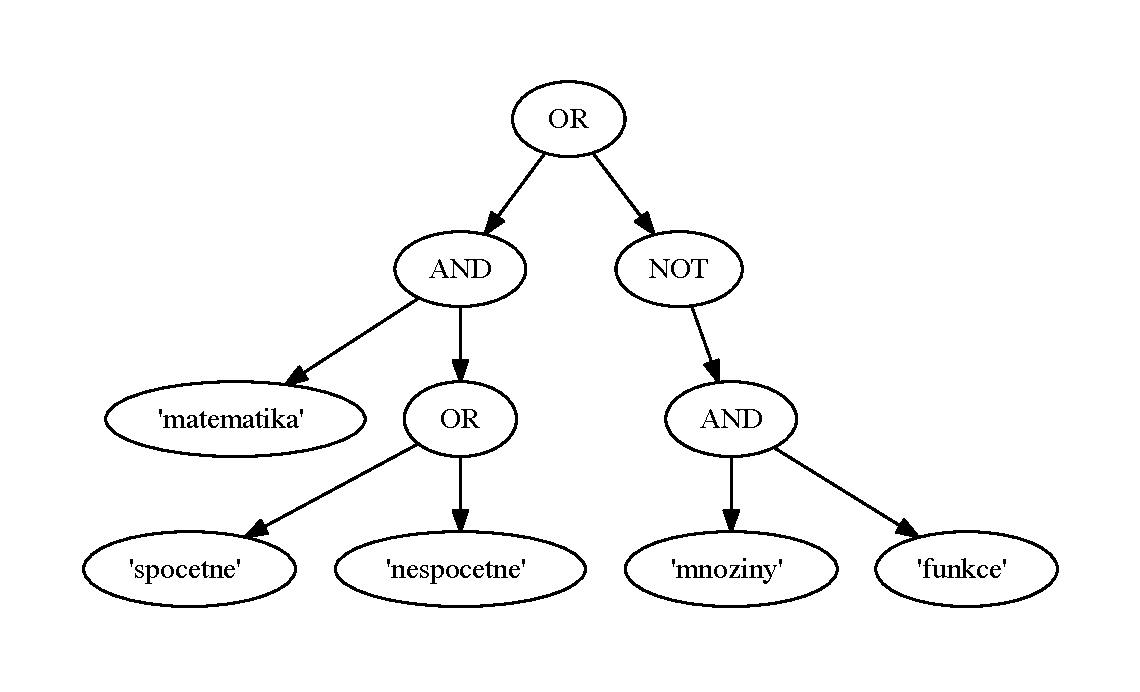
\includegraphics[width=14cm]{obrazky/syntactic_tree.pdf}
  \caption{Syntaktický strom}
  \label{fig:syntree}
\end{figure}

Nakonec celý výraz zjednodušíme -- odstraníme uzly, které obsahují stop slova, protože stop slova nepoužíváme při vyhledávání a převedeme slova na stemy. 

Více informací o parsování dotazu je například v \cite{compilers}.

\sssection{Vyhledání odpovídajících dokumentů}

Ve chvíli, kdy máme syntaktický strom, se můžeme pustit do hledání dokumentů. K tomu využijeme vybudovaný index, který nám umožňuje snadno zjistit, v jakých dokumentech se vyskytuje dané slovo. Pro účely popisu mechanismu si definujeme funkci $\getdocs$, která bere na vstupu dotaz (syntaktický strom) $Q$ a na výstupu vrací množinu dokumentů, které odpovídají zadanému dotazu. Tato funkce se bude chovat odlišně v závislosti na tom, jak vypadá dotaz $Q$. 

Dále označme $\alldoc$ množinu všech dokumentů a $\alpha$ a $\beta$ nechť označují nějaké dotazy. 

\begin{itemize}
\item Je-li $Q=s$, kde $s$ je nějaký stem, pak funkce $\getdocs$ vrátí množinu dokumentů, které obsahují daný stem, což vyčteme z indexu. Formálně to můžeme zapsat jako:
$$
\getdocs_s = \left\{d\in \alldoc\sep s\in d\right\}.
$$
\item Je-li dotaz ve tvaru Q = \uv{$\alpha$ AND $\beta$}, pak $\getdocs_Q = \getdocs_\alpha \cap \getdocs_\beta$.
\item Je-li dotaz ve tvaru Q = \uv{$\alpha$ OR $\beta$}, pak $\getdocs_Q = \getdocs_\alpha \cup \getdocs_\beta$.
\item Je-li dotaz ve tvaru Q = \uv{NOT $\alpha$}, pak $\getdocs_Q = \alldoc\setminus\getdocs_\alpha$.
\end{itemize}

Postupnou aplikací těchto pravidel dostaneme množinu výsledných dokumentů $R$. V dalším kroku tyto dokumenty seřadíme podle relevance. 

\sssection{Seřazení dokumentů}

V současné chvíli máme množinu dokumentů $\getdocs_Q$. Aby byl vyhledávač smysluplný, měl by tyto dokumenty seřadit podle toho, jak relevantní dané dokumenty vzhledem k položenému dotazu jsou. To je obecně nelehký úkol. Ve vyhledávači je pak použit standardní $\tfidf$ algoritmus popsaný v části \ref{tfidf}

Abychom mohli ohodnotit jednotlivé dokumenty, potřebujeme znát slova, vůči kterým máme dokumenty ohodnocovat. Odstraníme tak z dotazu všechny operátory a dostaneme množinu všech slov $S$. Vůči těmto slovům budeme dokumenty hodnotit. 

K tomu už využijeme $\tfidf$ algoritmus -- pro každé slovo z množiny $S$ a pro každý dokument z množiny $\getdocs_Q$ spočítáme jeho $\tfidf$ skóre; poté tato skóre sečteme a dokumenty seřadíme sestupně podle tohoto skóre. Skóre $\score_{d,S}$ dokumentu $d$ tak udává vzorec:
$$\score_{d,S}=\sum_{s\in S} \tfidf_{s, d}.$$

Toto základní skóre ještě dále upravíme podle toho, zda se klíčová slova z dotazu nevyskytují v důležitých částech dokumentu, konkrétně jde o název, adresu a popisek stránky. Za každé klíčové slovo, které se vyskytuje v názvu stránky $d$ nebo v adrese stránky, ztrojnásobíme hodnotu $\score_{d,S}$. Za každé klíčové slovo, které se vyskytuje v popisu stránky $d$, zdvojnásobíme hodnotu $\score_{d,S}$. Ve výsledku tak dostáváme funkci $\rank$, která nejprve vypočte hodnotu $\score_{d,S}$ a poté aplikuje pravidla o ztrojnásobení a zdvojnásobení. Funkce $\rank$ bere na vstupu dva parametry: dokument $d$, pro který počítáme skóre a slova $S$ z dotazu $Q$.

\begin{figure}
\begin{algorithmic}[1]
\Function{rank}{$d, S$}
    \State $score \gets \score_{d, S}$
    \ForAll{$s \in S$} 
    	\If{$s \in \mbox{title}(d) \quad\vee\quad s \in \mbox{url}(d)$}
    		\State $score \gets score \cdot 3$
    	\EndIf
    	\If{$s \in \mbox{description}(d)$}
    		\State $score \gets score \cdot 2$
    	\EndIf
    \EndFor
    \State \Return $score$
\EndFunction
\end{algorithmic}
\end{figure}



Nyní seřadíme dokumenty $\getdocs_Q$ do $n$-tice $\addsp{d_1, d_2, \ldots, d_n}$, kde 
$$n=\left|\getdocs_Q\right|\quad\mbox{a}\quad \bigcup_{i=1}^n d_i=\getdocs_Q$$ 
tak, aby platilo $\rank_{d_1, S} \ge \rank_{d_2, S} \ge \ldots \ge \rank_{d_n, S}$. Tato seřazená $n$-tice je výstupem algoritmu vyhledávání.

Idea a postup řazení dokumentů je popsán v \cite{introir}, včetně zvýhodňování určitých částí dokumentu. 





%%%%%%%%%%%%%%%%%%%%%%%%%%%%%%%%%%%%%%%%%%%%%%%%%%%%%%%%%%%%%%
%%%%%%%%%%%%%%%%%%%% FCA ČÁST VYHLEDÁVAČE %%%%%%%%%%%%%%%%%%%%
%%%%%%%%%%%%%%%%%%%%%%%%%%%%%%%%%%%%%%%%%%%%%%%%%%%%%%%%%%%%%%

\newpage
\section{Formální konceptuální analýza}
Formální konceptuální analýzu budeme používat jako matematický základ pro hledání souvisejících dotazů. V této kapitole bude popsána nezbytná teorie FCA. 

Základní teorie kolem FCA byla poprvé představena roku 1982 v článku \uv{Restructuring Lattice Theory: An Approach Based on Hierarchies of Concepts}, jehož autorem je německý matematik Rudolf Wille, viz \cite{wille}.

\ssection{Neformální úvod do formální konceptuální analýzy}
Formální konceptuální analýza pracuje s tabulkovými daty. V řádcích máme objekty, ve sloupcích máme atributy objektů. Obsahem každé buňky je pak informace, zda daný objekt má daný atribut. Tato informace je binární, daný objekt buď daný atribut má, nebo nemá. 

V tabulce \ref{tab.con1} je příklad takových tabulkových dat. V řádcích se nachází objekty -- živočichové či rostliny. Ve sloupcích pak jednotlivé atributy, což jsou nějaké vlastnosti, které dané objekty mohou mít. Pod tabulkou je legenda k jednotlivým atributům. Například první atribut $a$ je \uv{potřebuje k životu vodu}. Každý živočich a každá rostlina potřebuje k životu vodu, takže v celém sloupečku je křížek. Druhý atribut $b$ je \uv{žije ve vodě}. Zde už není křížek všude, takový pes ve vodě nežije. 


Takové tabulce s daty říkáme \strong{kontext}. V tomto kontextu pak hledáme shluky potenciálně zajímavých dat. Shlukem může být například množina $\adds{\mbox{Cejn, Žába, Pes}}$, protože všechna tato zvířata sdílí společné atributy $\adds{a, g, h}$ -- potřebují vodu k životu, mohou se pohybovat a mají končetiny. Zároveň platí, že cejn, žába a pes žádné další společné atributy nesdílí a podobně u atributů: žádný další objekt už nemá právě tyto tři společné vlastnosti. Takové dvě množiny objektů a atributů pak tvoří \strong{koncept}. Množinu objektů konceptu nazýváme \strong{extent} a množinu atributů \strong{intent}. 


\begin{table}
\begin{center}
\begin{tabular}{r|ccccccccc}
\toprule
&a&b&c&d&e&f&g&h&i\\
\midrule
Pijavice&\yes&\yes&&&&&\yes\\
Cejn&\yes&\yes&&&&&\yes&\yes\\
Žába&\yes&\yes&\yes&&&&\yes&\yes\\
Pes&\yes&&\yes&&&&\yes&\yes&\yes\\
Bodlák&\yes&\yes&&\yes&&\yes\\
Rákosí&\yes&\yes&\yes&\yes&&\yes\\
Fazole&\yes&&\yes&\yes&\yes\\
Kukuřice&\yes&&\yes&\yes&&\yes\\
\bottomrule
\end{tabular}
\end{center}
\caption{Formální kontext, zdroj: \cite{belfcaskr}} \label{tab.con1}

\begin{center}
$a$: potřebuje k životu vodu, $b$: žije ve vodě, $c$: žije na zemi,\\ $d$: potřebuje chlorofyl, $e$: dvouděložná rostlina, $f$: jednoděložná rostlina,\\ $g$: může se pohybovat, $h$: má končetiny, $i$: kojí potomky
\end{center}
\end{table}

Když se podíváme na tabulku, zjistíme, že koncept je tvořený křížky, které dohromady tvoří \uv{rozházený obdélník}. Pokud bychom ale sloupce, které reprezentují množinu společných atributů, přesunuly k sobě, získali bychom hezký obdélník (v tomto případě dokonce čtverec). Koncept je zvýrazněný v tabulce \ref{tab.con2} Vždy nás zajímá maximální obdélník, tj. pokud existuje objekt nebo atribut, který můžeme přidat a opět získáme obdélník, přidáme ho. 

\begin{table}
\begin{center}
\begin{tabular}{r|ccccccccc}
\toprule
&b&c&d&e&f&g&h&a&i\\
\midrule
Pijavice&\yes&&&&&\yes&&\yes\\
Cejn&\yes&&&&&\fyes&\fyes&\fyes\\
Žába&\yes&\yes&&&&\fyes&\fyes&\fyes\\
Pes&&\yes&&&&\fyes&\fyes&\fyes&\yes\\
Bodlák&\yes&&\yes&&\yes&&&\yes\\
Rákosí&\yes&\yes&\yes&&\yes&&&\yes\\
Fazole&&\yes&\yes&\yes&&&&\yes\\
Kukuřice&&\yes&\yes&&\yes&&&\yes\\
\bottomrule
\end{tabular}
\end{center}
\caption{Formální kontext se zvýrazněným konceptem} \label{tab.con2}
\end{table}


To samozřejmě není jediný koncept, který kontext obsahuje. Ve skutečnosti tento kontext obsahuje 19 konceptů. Zkusíme si najít další. Existuje něco, co žije na zemi i ve vodě? Hledáme tak objekty, které mají atributy $\adds{b, c}$. Pohledem do tabulky zjistíme, že tyto vlastnosti má žába a rákosí. Nicméně ještě jsme nenalezli koncept, protože nevíme, jestli náhodou tyto objekty nesdílí ještě nějaký další atribut. Vzhledem k tomu, že všechny objekty mají atribut $a$, musíme ho přidat do množiny atributů. Tím už získáme koncept s objekty $\adds{\mbox{žába, rákosí}}$ a atributy $\adds{a, b, c}$.

Řekli jsme, že formální konceptuální analýza zároveň řeší i hierarchii shluků. Ta se řeší pomocí relace inkluze. Můžeme říci, že koncept, který se skládá z extentu $\adds{\mbox{pijavice, cejn, žába a pes}}$ a intentu $\adds{a, g}$ je obecnější než koncept $\adds{\mbox{cejn, žába a pes}}$ a $\adds{a, g, h}$. 

První koncept můžeme pojmenovat \uv{pohybující se živočichové}, druhý koncept by byl \uv{živočichové, kteří k pohybu využívají končetiny}. Druhý koncept obsahuje všechny atributy jako první koncept, plus jeden navíc -- ten nějakým způsobem konkretizuje tento koncept. U objektů to platí naopak. Druhý koncept má více atributů, ale méně objektů. To je logické, pokud zvýšíme počet atributů, které objekty musí mít, zvýšíme tím na objekty nároky a objektů ubude. 

Tím už se blížíme k definici uspořádání konceptů. Pokud je nějaký koncept konkrétnější než jiný, řekneme, že je menší. Koncept $A$ je konkrétnější než koncept $B$, zapíšeme $A < B$, pokud je extent konceptu $A$ vlastní podmnožinou extentu konceptu $B$. Tím máme definováno uspořádání, kterým můžeme uspořádat všechny koncepty. Přesnější popis bude v následující kapitole. 

\ssection{Formální zavedení FCA}

Všechny definice a všechny věty z této kapitoly jsou citovány z \cite{belfcaskr}. Další materiály o FCA: \cite{fcabook}, \cite{fcaslajdy1}, \cite{fcaslajdy2}, \cite{fcaslajdy3}.

\sssection{Základní pojmy}
\begin{mydef}[Formální kontext]
Formální kontext je trojice $\addsp{X, Y, I}$, kde $X$ je neprázdná množina objektů, $Y$ je neprázdná množina atributů a $I$ je binární relace mezi $X$ a $Y$, tj. $I\subseteq X\times Y$.
\end{mydef}

V předchozím příkladě byla množina $X$ rovna živočichům a rostlinám a množina $Y$ byla rovna vlastnostem těchto živočichů a rostlin. Relace $I$ pak vyznačuje, zda má objekt $x$ atribut $y$. Objekt $x$ má atribut $y$ právě tehdy, když $\addsp{x, y}\in I$. Formální kontext, jak jsme viděli, může být reprezentován pomocí tabulky. 

\begin{mydef}[Šipkové operátory]
Pro kontext $\context$ definujeme operátory $\up:2^X\rightarrow2^Y$ a $\down:2^Y\rightarrow2^X$ tak, že pro každé $A\subseteq X$ a $B\subseteq Y$:
\begin{eqnarray}
A\up&=&\adds{y\in Y\sep \foreach x \in A: \addsp{x, y}\in I}\\
B\down&=&\adds{x\in X\sep\foreach y\in B:\addsp{x, y} \in I}
\end{eqnarray}
\end{mydef}

Tyto operátory umožňují zjistit společné vlastnosti. Operátor $\up$ nám zjistí všechny atributy, které mají všechny objekty v $A$ společné. Operátor $\down$ nám zjistí všechny objekty, které sdílí všechny atributy z $B$. 

Pokud se vrátíme ke kontextu v tabulce \ref{tab.con1}, tak:

\begin{eqnarray*}
\adds{\mbox{Žába}}\up&=&\adds{a, b, c, g, h}\\
\adds{\mbox{Fazole, Bodlák}}\up&=&\adds{a, d}\\
\adds{\mbox{Pijavice, Pes, Kukuřice}}\up&=&\adds{a}\\
X\up&=&\adds{a}\\
\adds{c, d}\down&=&\adds{\mbox{Rákosí, Fazole, Kukuřice}}\\
\adds{f, g}\down&=&\emptyset\\
\adds{b}\down&=&\adds{\mbox{Pijavice, Cejn, Žába, Bodlák, Rákosí}}
\end{eqnarray*}


\begin{mydef}[Formální koncept]
Formální koncept v kontextu $\context$ je dvojice $\AB$, $A\subseteq X$, $B\subseteq Y$ tak, že:
$$A\up=B\logand B\down =A.$$

Množině $A$ říkáme \uv{extent} a množině $B$ \uv{intent}.
\end{mydef}

Takto definovaný formální koncept odpovídá naší předchozí představě o konceptu. Pokud jsme měli danou množinu objektů, pak jsme našli sdílené atributy. K těmto sdíleným atributům jsme následně nalezli objekty, které všechny tyto atributy sdílí, což mohlo být více objektů, než jaké jsme měli na začátku. Ve chvíli, kdy se k těmto objektům pokusíme najít sdílené atributy, nenalezneme již žádný nový.

V tabulce \ref{tab.con1} tak můžeme najít například koncept 
$$\addsp{\adds{\mbox{Cejn, Žába}}, \adds{a, b, g, h}},$$ 
protože 
$$\adds{\mbox{Cejn, Žába}}\up=\adds{a, b, g, h}\quad \logand \quad \adds{a, b, g, h}\down=\adds{\mbox{Cejn, Žába}}.$$


\sssection{Galoisova spojení}

Évariste Galois byl francouzský matematik 19. století. Je známý svou prací v oblasti moderní algebry a považuje se za zakladatele teorie grup. Bohužel zemřel již ve svých dvaceti letech, když se účastnil střeleckého souboje. My využijeme Galoisovo spojení jako základní matematickou strukturu pro FCA.

\begin{mydef}[Galoisovo spojení] \label{def.gal}
Galoisovo spojení mezi množinami $X$ a $Y$ je dvojice zobrazení $\addsp{f,g}$, $f:2^X\rightarrow2^Y$ a $g:2^Y\rightarrow2^X$, která pro všechna $A, A_1, A_2\subseteq X$ a $B, B_1, B_2\subseteq Y$ splňují:

\begin{eqnarray}
&&A_1\subseteq A_2\implies f(A_2)\subseteq f(A_1)\label{eq.gal1}\\
&&B_1\subseteq B_2\implies g(B_2)\subseteq g(B_1)\\
&&A\subseteq g(f(A))\label{eq.gal2}\\
&&B\subseteq f(g(B))
\end{eqnarray}
\end{mydef}

Galoisovo spojení má jednoduchou interpretaci, kterou si můžeme ukázat na příkladu herců a filmů. Nechť množina $X$ je množina všech herců a hereček a množina $Y$ všech filmů. 

Zobrazení $f$ nám pro danou podmnožinu herců $A$ vrací množinu filmů, ve kterých všichni herci z množiny $A$ hráli. Zobrazení $g$ naopak vrací pro podmnožinu filmů $B$ takovou množinu herců, kteří hráli ve všech filmech v množině $B$. Výsledkem $f(\adds{\mbox{Bruce Willis}})$ je množina všech filmů, ve kterých hrál Bruce Willis. Výsledkem $g(\adds{\mbox{Pelíšky; Dobrá zpráva; Pasti, pasti, pastičky}})$ je množina herců a hereček, kteří hráli ve všech těchto filmech: $\adds{\mbox{Miroslav Donutil, Eva Holubová}}$.

Vlastnosti zmíněné v definici \ref{def.gal} už jsou pak velmi přirozené. Vlastnost \ref{eq.gal1} říká, že pokud máme skupiny herců $A_1=\adds{\mbox{Johnny Depp}}$ a $A_2=\adds{\mbox{Johnny Depp, Bruce Lee}}$, tak můžeme očekávat, že pouze Depp hrál ve více filmech než Depp spolu s Leem. Filmy, ve kterých spolu hráli Depp a Lee jsou určitě podmnožinou filmů, kde hrál pouze Depp.

Vlastnost \ref{eq.gal2} zase říká, že pokud nalezneme všechny filmy, ve kterých hrál Johnny Depp a poté nalezneme všechny herce, kteří hráli ve všech těchto filmech, tak mezi těmito herci musí být Johnny Depp. Ostatní dvě vlastnosti říkají duálně totéž. 

\begin{mydef}[Pevné body Galoisova spojení]
Pro Galoisovo spojení $\addsp{f, g}$ mezi množinami $X$ a $Y$ definujeme množinu
$$
\fix(\addsp{f,g})=\adds{\addsp{A,B}\in 2^X\times2^Y\sep f(A)=B, g(B)=A}.
$$
Tuto množinu nazýváme množinu pevných bodů spojení $\addsp{f,g}$. 
\end{mydef}

Pevným bodem je například dvojice 
\begin{eqnarray*}
A&=&\adds{\mbox{Miroslav Donutil, Eva Holubová}},\\
B&=& \adds{\mbox{Pelíšky; Dobrá zpráva; Pasti, pasti, pastičky}}.
\end{eqnarray*}

Donutil s Holubovou spolu nehráli v žádném dalším filmu, kromě těchto tří. A zároveň v těchto třech filmech spolu nehráli žádní jiní herci než Donutil a Holubová. 

\begin{theorem}[Zřetězení Galoisových spojení]\label{th.chain}
Pro Galoisovo spojení $\addsp{f,g}$ mezi $X$ a $Y$ a pro všechna $A\subseteq X$ a $B\subseteq Y$ platí:

\begin{eqnarray}
f(A)&=&f(g(f(A)))\\
g(B)&=&g(f(g(B)))
\end{eqnarray}
\qed\end{theorem}

Toto je zajímavá vlastnost. Na začátku máme množinu herců $A$. Nalezneme filmy, ve kterých tito herci hráli. Tím získáme $f(A)$. Dále nalezneme herce, kteří hráli ve všech těchto nalezených filmech. Tam se určitě objeví herci z $A$, viz definici \ref{def.gal}, ale mohou se tam objevit i další herci. Tím získáme hodnotu $g(f(A))$. Nakonec zpátky spočítáme filmy, ve kterých tito herci hráli. Musíme nutně získat množinu filmů $f(A)$, protože $g(f(A))$ jsou právě herci, kteří hrají všech filmech z $f(A)$.

\begin{mydef}[Uzávěrový operátor]\label{def.clop}
Uzávěrový operátor $C$ na množině $X$ je zobrazení $C: 2^X\rightarrow2^X$, které pro každé $A, A_1, A_2\subseteq X$ splňuje:
\begin{eqnarray}
&&A\subseteq C(A),\\
&&A_1\subseteq A_2\implies C(A_1) \subseteq C(A_2),\\
&&C(A) = C(C(A)).
\end{eqnarray}
\end{mydef}

\begin{mydef}[Pevné body uzávěrového operátoru]
Pro uzávěrový operátor $C: 2^X\rightarrow2^X$ pojmenujeme množinu
$$
\fix(C)=\adds{A\subseteq X\sep C(A)=A}
$$
jako množinu pevných bodů uzávěrového operátoru $C$.
\end{mydef}

\begin{theorem}[Od Galoisova spojení k uzávěrovému operátoru]\label{th.galcl}
Nechť $\addsp{f,g}$ je Galoisovo spojení mezi $X$ a $Y$. Potom $C_X=f\circ g$ je uzávěrový operátor na $X$ a $C_Y=g\circ f$ je uzávěrový operátor na $Y$. 
\qed\end{theorem}

Zápis $f \circ g$ značí skládání množin ve smyslu $(f \circ g)(x) = g(f(x))$.

Pevným bodem uzávěrového operátoru nad množinou herců rozumíme takovou množinu herců, kteří spolu hráli v určitých filmech, ale \strong{žádní jiní herci už v těchto filmech nehráli}. Poslední vlastnost je pro pevný bod klíčová. 

Je například množina $\adds{\mbox{Danny Glover, Mel Gibson}}$ pevným bodem? Věta \ref{th.galcl} nám říká, jak postupovat, pokud pevný bod chceme nalézt. Jako první vypočteme $f(\adds{\mbox{Danny Glover, Mel Gibson}})$. Tím získáme množinu filmů, ve kterých herci hráli spolu, tj. $\adds{\mbox{Smrtonosná zbraň 1, 2, 3, 4}}$. Nyní zpět zjistíme herce, kteří hráli v těchto filmech, spočítáme $g(\adds{\mbox{Smrtonosná zbraň 1, 2, 3, 4}})$. Kromě Gibsona a Glovera se tam objeví ještě Mary Ellen Trainor: $\adds{\mbox{Danny Glover, Mel Gibson, Mary Ellen Trainor}}$. Tato množina herců a hereček je už pevným bodem. 

Uzávěrový operátor si můžeme ukázat i na úplně jiném příkladě, doplnění rovinného útvaru na nejmenší konvexní útvar. Máme-li tak nějaký útvar v rovině, který není konvexní, například klasický obrázek hvězdy, uzávěrový operátor ho doplní tak, aby z něj vznikl konvexní útvar a aby tento nový útvar byl nejmenší. Na tomto operátoru si můžeme ilustrovat podmínky v definici \ref{def.clop}.

První vlastnost říká, že původní útvar bude vždy podmnožinou uzavřeného útvaru. Původní rovinný útvar bude vždy celý obsažen v konvexním útvaru, který ho má obalovat -- uzavřením pouze \uv{přidáme} původnímu útvaru body tak, aby vznikl konvexní útvar. Druhá vlastnost říká, že pokud máme dva různé útvary, přičemž jeden je zanořený ve druhém, tak i jejich obaly budou zanořené. Poslední vlastnost říká, že obalem obalu je tentýž obal. Pokud obalíme hvězdu konvexním útvarem, pro příklad pravidelným pětiúhelníkem, tak obalem tohoto pětiúhelníku bude tentýž pětiúhelník.

\begin{theorem}
Nechť $\addsp{f,g}$ je Galoisovo spojení mezi $X$ a $Y$. Pak pro každé $A_j\subseteq X, j\in J$ a $B_j\subseteq Y, j\in J$ platí:

\begin{eqnarray}
f(\bigcup_{j\in J}A_j)&=&\bigcap_{j\in J}f(A_j)\\
g(\bigcup_{j\in J}B_j)&=&\bigcap_{j\in J}g(B_j)
\end{eqnarray}
\qed\end{theorem}

\begin{theorem}[Šipkové operátory tvoří Galoisovo spojení]
Pro formální kontext $\context$ tvoří dvojice $\addsp{\up, \down}$ Galoisovo spojení mezi $X$ a $Y$.
\qed\end{theorem}

Předchozí věta je důležitým výsledkem. Odpovídá nám na otázku, jak jednoduše počítat extenty a intenty k libovolným podmnožinám objektů či atributů. Protože pro kontext $\context$ je $\addsp{\up, \down}$ Galoisovo spojení, platí, že zobrazení $\up\circ\down$ je uzávěrový operátor na množině $X$, tj. na množině objektů. 

Máme-li množinu objektů $A \subseteq X$, pak uzavřením $A\updown$ získáme pevný bod operátoru, což je zároveň extent nějakého konceptu. Podobně pokud máme množinu atributů $B \subseteq Y$, pak uzavřením $B\downup$ získáme intent nějakého konceptu. 

Pokud si spočítáme extent jako $A\updown$, můžeme intent tohoto konceptu zjistit tak, že ještě jednou spočítáme $\up$, dostaneme tak množinu $A^{\uparrow\downarrow\uparrow}$. Nicméně z věty \ref{th.chain} víme, že $A\up = A^{\uparrow\downarrow\uparrow}$, takže intent je zároveň rovný $A\up$. Jakýkoliv pár tvaru $\addsp{A\updown, A\up}$, kde $A\subseteq X$, tvoří formální koncept. 

Můžeme si také označit množinu všech extentů jako $\ext$ a množinu všech intentů jako $\intfca$:

\begin{eqnarray}
\ext(X, Y, I)&=&\fix(\updown),\\
\intfca(X, Y, I)&=&\fix(\downup).
\end{eqnarray}

Dále si označíme množinu všech konceptů kontextu $\addsp{X,Y,I}$:

\begin{eqnarray}
\lattice&=&\adds{\addsp{A, A\up}\sep A\in\ext(X,Y,I)},\\
\lattice&=&\adds{\addsp{B\down, B}\sep B\in\intfca(X,Y,I)}.
\end{eqnarray}


\sssection{Konceptuální svaz}
\begin{mydef}[Uspořádání konceptů]
\label{def.order}
O konceptech $\addsp{A_1, B_1}, \addsp{A_2, B_2}$ kontextu $\context$ řekeneme, že
$$\addsp{A_1, B_1}\le\addsp{A_2, B_2}\quad\pravekdyz\quad A_1\subseteq A_2 \quad(B_2\subseteq B_1).$$
\end{mydef}

Relaci menší nebo rovno mezi koncepty můžeme interpretovat jako relaci \uv{být konkrétnější koncept}. Pokud pro koncepty platí $\addsp{A_1, B_1}\le\addsp{A_2, B_2}$, pak koncept $\addsp{A_1, B_1}$ je konkrétnější než koncept $\addsp{A_2, B_2}$. 

\begin{theorem}[Extenty, intenty a formální koncepty]Některé důležité vlastnosti množin extentů, intentů a konceptů:
\begin{enumerate}
	\item $\addsp{\ext(X,Y,I), \subseteq}$ a $\addsp{\intfca(X,Y,I), \subseteq}$ jsou (částečně) uspořádáné množiny. 
	\item $\addsp{\ext(X,Y,I), \subseteq}$ a $\addsp{\intfca(X,Y,I), \subseteq}$ jsou duálně isomorfní. Tj. existuje zobrazení $f: \ext(X,Y,I)\rightarrow\intfca(X,Y,I)$ takové, že $A_1\subseteq A_2$ platí právě tehdy, když $f(A_2)\subseteq f(A_1)$.
	\item $\addsp{\lattice, \le}$ je isomorfní s $\addsp{\ext(X,Y,I), \subseteq}.$
\end{enumerate}
\qed\end{theorem}

\begin{mydef}[Svaz]
Nechť $\addsp{X, \le}$ je uspořádaná množina. Pokud pro každé $x,y\in X$ existuje $\sup(x,y)$ a $\inf(x,y)$, pak $\addsp{X, \le}$ nazveme svaz. Pokud můžeme nalézt infima a suprema pro jakoukoliv podmnožinu množiny $X$, pak se jedná o úplný svaz. 
\end{mydef}

Uspořádaná množina tak je svazem, pokud dokážeme ke každým dvěma prvkům množiny nalézt jejich infimum a supremum. Příkladem jednoduchého svazu mohou být reálná čísla s klasickým uspořádáním. Pak platí, že pro $x,y\in\mathbb{R}$: $\sup(x,y)=\max(x,y)$ a $\inf(x,y)=\min(x,y)$.

Dalším příkladem svazu je $\addsp{2^{\mathbb{N}}, \subseteq}$, množina všech podmnožin přirozených čísel s uspořádáním podle množinové inkluze. Platí pak, že pro $X, Y \in 2^{\mathbb{N}}$ máme $\sup(X, Y) = X \cup Y$ a $\inf(X, Y) = X \cap Y$.

\begin{mydef}[Konceptuální svaz]
Pro kontext $\context$ máme definovanou množinu všech formálních konceptů $\lattice$ z $\context$. Tedy
$$\lattice=\adds{\addsp{A, B}\in 2^X\times 2^Y\sep A\up=B\logand B\down=A}.$$

Dvojice $\addsp{\lattice, \le}$ se nazývá konceptuální svaz. 
\end{mydef}

K tomu, abychom dokázali, že $\addsp{\lattice, \le}$ je skutečně svaz, musíme dokázat, že pro každé dva koncepty $c_1, c_2\in\addsp{\lattice, \le}$ existuje v tomto svazu jejich supremum a infimum. Vrátíme se ještě k obecnému uzávěrovému operátoru. 

\begin{theorem}[Systém pevných bodů uzávěrového operátoru]\label{th.sysfix}
Mějme uzávěrový operátor $C$ na množině $X$. Pak uspořádaná množina $\addsp{\fix(C), \le}$ pevných bodů tohoto operátoru je úplný svaz, kde infima a suprema získáme

\begin{eqnarray}
\biginf_{j\in J}A_j&=&\bigcap_{j\in J}A_j,\label{eq.clinf}\\
\bigsup_{j\in J}A_j&=&C(\bigcup_{j\in J}A_j).\label{eq.clsup}
\end{eqnarray}
\qed\end{theorem}

Ukážeme si na příkladu myšlenku důkazu. Rovnice \ref{eq.clinf} říká, že pokud máme dva pevné body uzávěrového operátoru a provedeme jejich průnik, pak opět získáme pevný bod a tento bod bude zároveň infimem původních dvou bodů (rovnice je ve skutečnosti obecnější a povoluje libovolně velkou množinu pevných bodů, ne jen dva).

Vrátíme se k příkladu uzávěrového operátoru, který uzavíral rovinný útvar na nejmenší konvexní útvar. Představme si dva konvexní útvary, například dva kruhy, které se protínají. Jejich průnikem pak bude jistě konvexní útvar. 

Zajímavější je v tomto případě rovnice \ref{eq.clsup}, kde počítáme supremum. Očekávali bychom, že bude stačit pevné body pouze sjednotit a dostaneme opět pevný bod. Nicméně tomu tak není. Abychom dostali pevný bod, musíme sjednocení bodů ještě znovu uzavřít. Když se vrátíme ke kruhům -- sjednotíme-li dva protínající se kruhy, získáme útvar, který není konvexní. Abychom získali konvexní útvar, musíme tyto dva sjednocenné útvary opět uzavřít. 

Nyní bychom měli ukázat, že $\biginf_{j\in J}A_j$ je skutečně rovno $\bigcap_{j\in J}A_j$. Už víme, že $\bigcap_{j\in J}A_j$ je také pevný bod. Z principu platí, že $\bigcap_{j\in J}A_j$ je menší nebo rovno než všechna $A_j$. Pokud si dále vezmeme množinu všech $B\in\fix(C)$, která jsou menší než všechna $A_j$, tak platí, že $\bigcap_{j\in J}A_j$ je větší nebo rovno než všechna tato $B$. Je to tedy největší prvek spodní závory množiny $\adds{A_j}$. 

Pokud to vztáhneme na příklad: největší konvexní útvar, který je obsažen ve dvou rovinných útvarech, je právě průnik těchto dvou útvarů. Jakýkoliv větší útvar, nebo stejně velký, ale jinam umístěný, nebude obsažen v alespoň jednom z útvarů a jakýkoliv menší útvar bude \dots\, menší. 

Dále ukážeme, že $C(\bigcup_{j\in J}A_j)$ je skutečně rovno $\bigsup_{j\in J}A_j$. Víme, že $C(\bigcup_{j\in J}A_j)$ je pevný bod. Dále víme, že $C(\bigcup_{j\in J}A_j)$ je větší nebo roven než všechna $A_j$, takže musí být větší nebo roven než supremum $\bigsup_{j\in J}A_j$, tj. $\bigsup_{j\in J}A_j\subseteq C(\bigcup_{j\in J}A_j)$. 

Dále platí, že $\bigsup_{j\in J}A_j\supseteq A_j$ pro všechna $j$ -- supremum systému množin musí být větší nebo rovno než každá množina systému. Z toho vyplývá, že $\bigsup_{j\in J}A_j\supseteq\bigcup_{j\in J}A_j$. Pokud je supremum větší nebo rovno než každá množina, pak je větší nebo rovno než sjednocení systému. Využijeme faktu, že uzavřením pevného bodu získáme tentýž pevný bod: pokud $B\in\fix(C)$, pak $B=C(B)$. Protože $\bigsup_{j\in J}A_j$ je pevným bodem, můžeme napsat $\bigsup_{j\in J}A_j=C(\bigsup_{j\in J}A_j)$. Upravíme předchozí inkluzi: 

\begin{eqnarray}
\bigsup_{j\in J}A_j&\supseteq&\bigcup_{j\in J}A_j\\
C(\bigsup_{j\in J}A_j)&\supseteq&C(\bigcup_{j\in J}A_j)\\
\bigsup_{j\in J}A_j&\supseteq&C(\bigcup_{j\in J}A_j)
\end{eqnarray}

Nejprve oba výrazy uzavřeme, čímž nezměníme platnost inkluze. Poté z levé strany odstraníme $C$, protože supremum už pevným bodem je. Dostali jsme tak
$$
\bigsup_{j\in J}A_j\supseteq C(\bigcup_{j\in J}A_j)\quad\mbox{a}\quad\bigsup_{j\in J}A_j\subseteq C(\bigcup_{j\in J}A_j)
$$

Z toho vyplývá, že $\bigsup_{j\in J}A_j=C(\bigcup_{j\in J}A_j)$.

\begin{mydef}[Supremálně a infimálně hustá množina]
Množinu $K\subseteq V$ nazveme supremálně hustou ve $V$ právě tehdy, když pro všechna $v \in V$ existuje $K^\prime\subseteq K$ takové, že $v=\bigsup K^\prime$. Každý prvek množiny $V$ je tak supremem nějakých prvků z $K$.

Duálně pro infimum: když pro všechna $v \in V$ existuje $K^\prime\subseteq K$ takové, že $v=\biginf K^\prime$.
\end{mydef}

\begin{theorem}[Hlavní věta konceptuálních svazů]
Věta má dvě části:
\begin{enumerate}
	\item Nechť $\lattice$ je kompletní svaz, kde suprema a infima získáme
	\begin{eqnarray}
	\biginf_{j\in J}\addsp{A_j, B_j}&=&\addsp{\bigcap_{j\in J}A_j, \addk{\bigcup_{j\in J}B_j}\downup},\label{eq.main1}\\
	\bigsup_{j\in J}\addsp{A_j, B_j}&=&\addsp{\addk{\bigcup_{j\in J}A_j}\updown,\bigcap_{j\in J}B_j}.
	\end{eqnarray}
	\item Dále, libovolný úplný svaz \textbf{V} $=\addsp{V,\le}$ je isomorfní k $\lattice$ právě tehdy, když existují zobrazení $\gamma: X\rightarrow V, \mu:Y\rightarrow V$ tak, že
	\begin{itemize}
		\item $\gamma(X)$ je supremálně hustá množina ve $V$ a $\mu(Y)$ je infimálně hustá množina v $V$,
		\item $\gamma(x)\le\mu(y)$ právě tehdy, když $\addsp{x,y}\in I$.
	\end{itemize}
\end{enumerate}
\qed\end{theorem}

% První část nám říká, jak hledat suprema a infima množiny konceptů. Důkaz první části hlavní věty o konceptuálních svazech:

% \begin{proof}
% Ověříme pouze rovnici \ref{eq.main1}, druhou rovnici bychom dokázali téměř stejně. Víme, že množiny extentů a intentů jsou pevnými body vzhledem k operátorům $\updown$ a $\downup$. Platí
% \begin{eqnarray}
% \addsp{\ext(X,Y,I), \subseteq}&=&\addsp{\fix(\updown),\subseteq}\\
% \addsp{\intfca(X,Y,I), \subseteq}&=&\addsp{\fix(\downup),\subseteq}
% \end{eqnarray}

% Dále víme, že konceptuální svaz $\addsp{\lattice, \le}$ je isomorfní s $\addsp{\ext(X,Y,I), \subseteq}$ a duálně isomorfní s $\addsp{\intfca(X,Y,I), \subseteq}$. Tedy infima v $\lattice$ korespondují s infimy v $\ext(X,Y,I)$ a supremy v $\intfca(X,Y,I)$. 

% Pro nás to znamená, že pokud máme množinu konceptů $\addsp{A_j, B_j}$ a cheme spočítat jejich infimum, stačí nám spočítat infimum extentů $\adds{A_j}$, čímž dostaneme extent konceptu, který je infimem konceptů $\addsp{A_j, B_j}$. Protože pracujeme s uzávěrovým operátorem $\updown$, můžeme, dle věty \ref{th.sysfix} spočítat infimum $\adds{A_j}$ jako obyčejný průnik: $\biginf_{j\in J}\adds{A_j}=\bigcap_{j\in J}A_j$. 

% Intent tohoto konceptu bychom mohli zapsat jako $(\bigcap_{j\in J}A_j)\up$. Ale můžeme využít faktu, že intent je supremum množiny $\adds{B_j}$, což je dle věty \ref{th.sysfix} rovno $\bigsup_{j\in J}B_j=(\bigcup_{j\in J}B_j)\downup$.
% \end{proof}


\sssection{Zobrazení konceptuálního svazu}
Už máme definované uspořádání na množině konceptů a víme, jak počítat suprema a infima, tak si ukážeme, jak takový konceptuální svaz vypadá. Vrátíme se k tabulce \ref{tab.con1}, kde byl zobrazen kontext s živočichy a rostlinami. Všechny koncepty v tomto kontextu jsou vypsány na obrázku \ref{fig.concepts} 

Tento svaz můžeme zobrazit klasickým Hasseovým diagramem, viz obrázek \ref{fig.lattice}

\begin{figure}
  \centering
  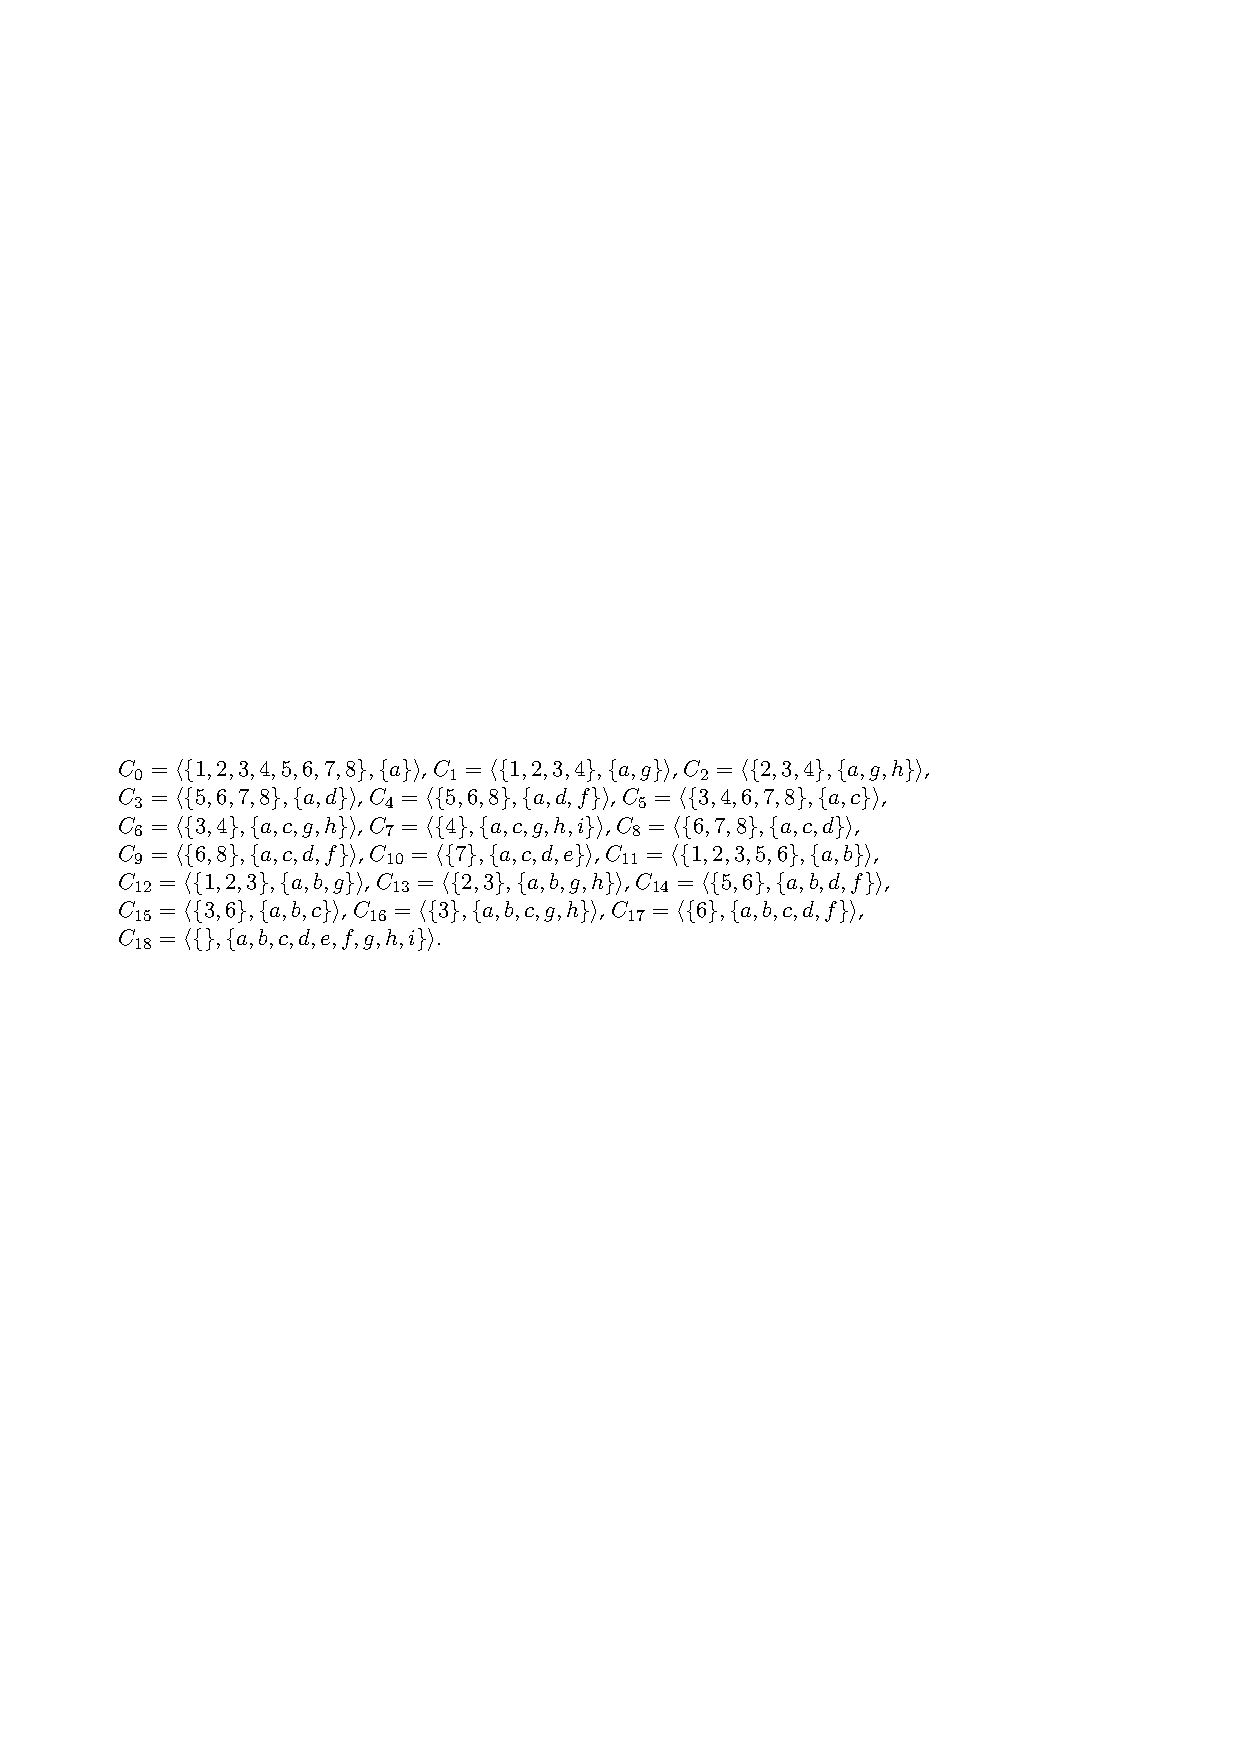
\includegraphics[width=14cm]{obrazky/koncepty.pdf}
  \caption{Všechny koncepty z kontextu v tabulce \ref{tab.con1}, zdroj: \cite{belfcaskr}}
  \label{fig.concepts}
\end{figure}

\begin{figure}
  \centering
  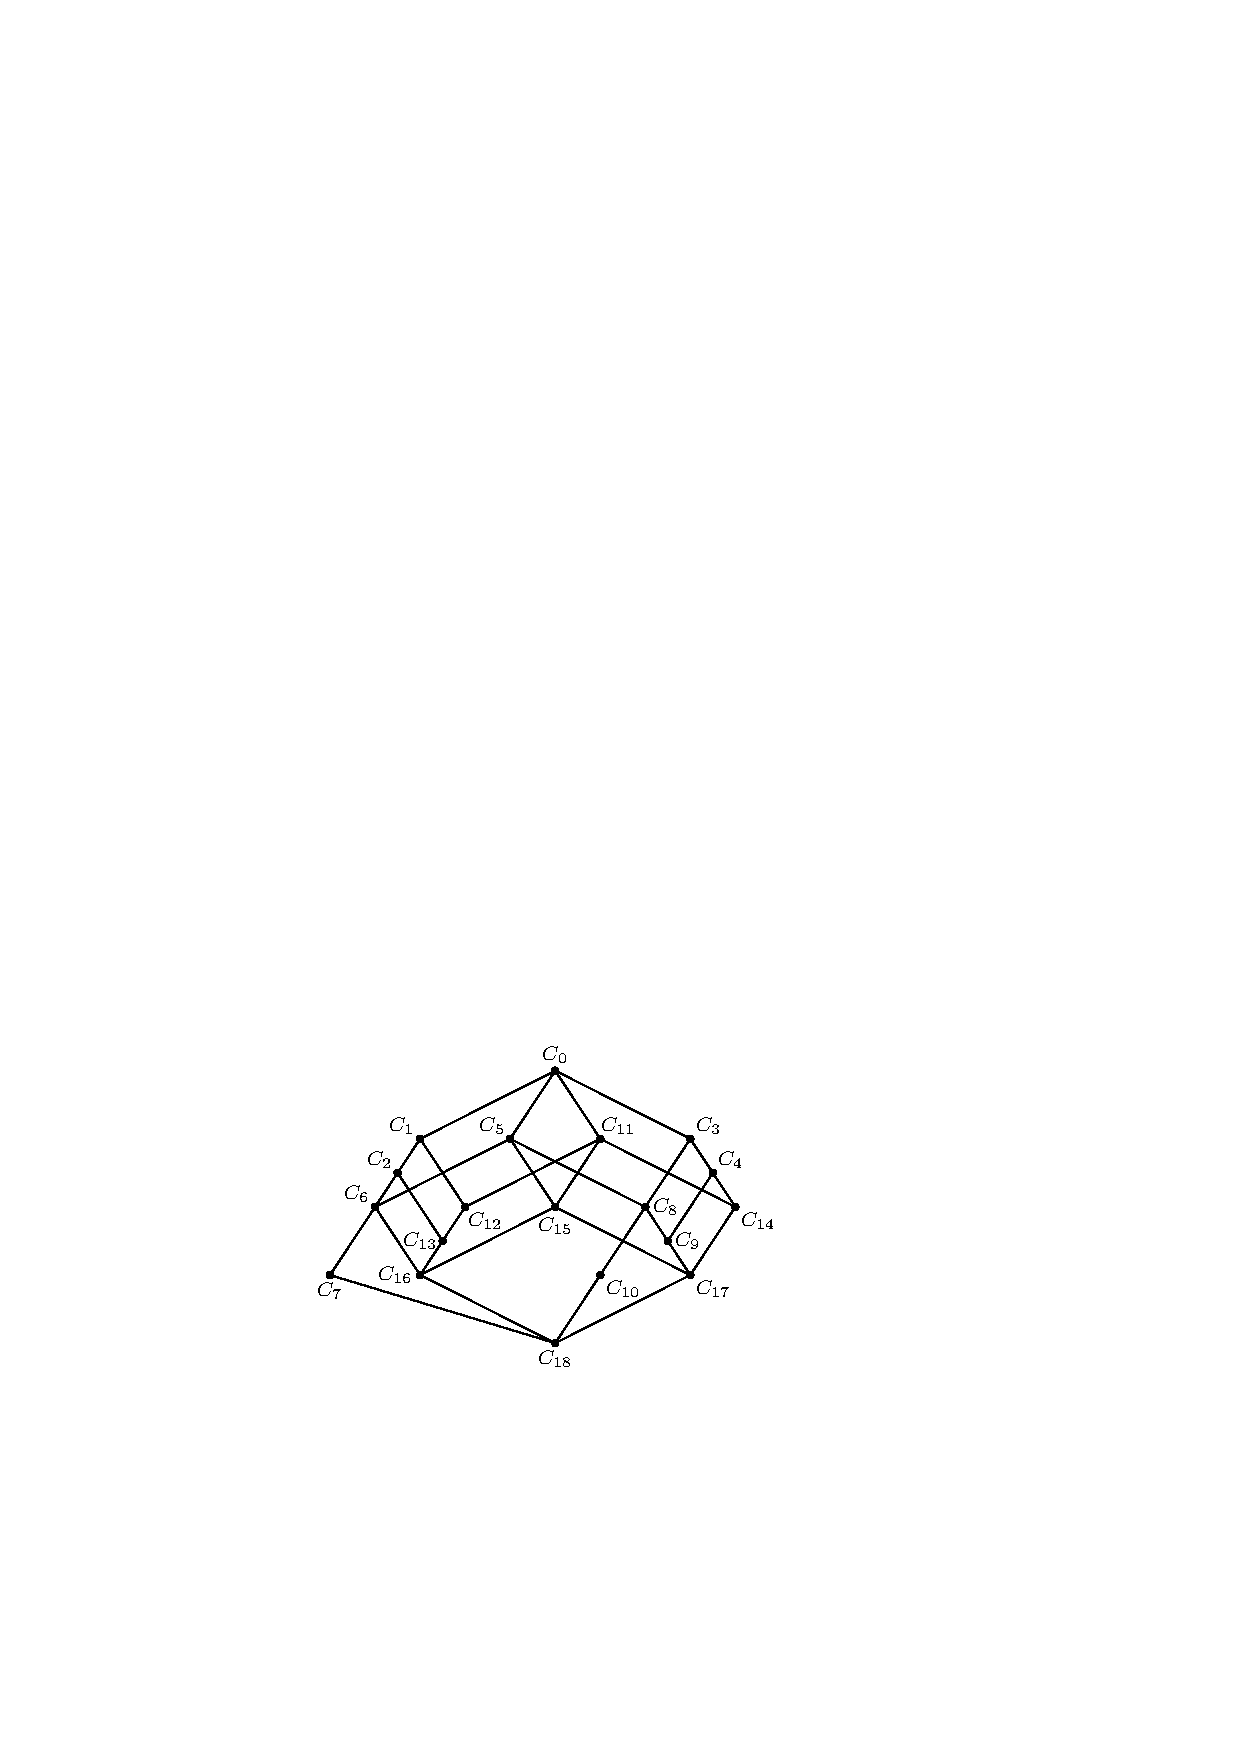
\includegraphics[width=14cm]{obrazky/svaz.pdf}
  \caption{Svaz, který vznikne z kontextu v tabulce \ref{tab.con1}, zdroj: \cite{belfcaskr}}
  \label{fig.lattice}
\end{figure}

Můžeme si na jednoduchých příkladech ukázat, jak se počítají infima a suprema. Vezměme si množinu konceptů $A=\adds{C_6, C_{15}}$. Z obrázku můžeme vyčíst, že infimum $A$ je rovno $C_{16}$ a supremum $C_5$. Nejdříve si zapíšeme koncepty včetně všech objektů a atributů
$$\biginf \adds{\addsp{\adds{3, 4}, \adds{a, c, g, h}}, \addsp{\adds{3, 6}, \adds{a, b, c}}}$$
a nyní spočítáme infimum množiny extentů těchto konceptů. Počítáme tak
$$
\biginf\adds{\adds{3, 4}, \adds{3, 6}} = \bigcap\adds{\adds{3, 4}, \adds{3, 6}} =\adds{3}
$$
Extent infima bude obsahovat pouze objekt číslo tři. Intent spočítáme podobně, pouze použijeme supremum a jeden uzávěrový operátor navíc: 
$$
\bigsup\adds{\adds{a,c,g,h}, \adds{a,b,c}}=\bigcup\adds{\adds{a,c,g,h}, \adds{a,b,c}}=\adds{a,b,c,g,h}
$$
Tuto množinu ještě musíme uzavřít:
$$
\adds{a,b,c,g,h}\downup=\adds{a,b,c,g,h}
$$
Žádný další atribut už ale nepřibyl. Získali jsme tak koncept $\addsp{\adds{3}, \adds{a,b,c,g,h}}$. Když se podíváme na výčet všech konceptů na obrázku \ref{fig.concepts}, zjistíme, že to opravdu odpovídá konceptu $C_{16}$, jak jsme očekávali. Supremum spočítáme podobně. 

















%%%%%%%%%%%%%%%%%%%%%%%%%%%%%%%%%%%%%%%%%%%%%%%%%%%%%%%%%%%%%%%%%%%%%%%%%%%
%%%%%%%%%%%%%%%%%%%% JAK VYHLEDÁVAČ TEORETICKY FUNGUJE %%%%%%%%%%%%%%%%%%%%
%%%%%%%%%%%%%%%%%%%%%%%%%%%%%%%%%%%%%%%%%%%%%%%%%%%%%%%%%%%%%%%%%%%%%%%%%%%
\newpage
\section{Hledání souvisejících dokumentů}
V této kapitole bude popsána druhá část vyhledávače, která se stará o nalezení souvisejících dotazů. 

\ssection{O co nám půjde}

\sssection{Motivace}

Pokud uživatel položí vyhledávači nějaký dotaz, vyhledávač odpoví nějakým seznamem dokumentů, které jsou podle něj nejvíce relevantní. Pokud má uživatel štěstí, bude v tomto seznamu dokument, který zrovna potřebuje najít. Pokud bude mít velké štěstí, pak bude tento dokument na předních místech v seznamu. 

Pokud ale toto štěstí mít nebude a dokument se mu nepodaří nalézt, musí uživatel nějakým způsobem přeformulovat svůj dotaz tak, aby vyhledávač vrátil jinou sadu výsledků. Obecně může upravit dotaz třemi různými způsoby. Může

\begin{enumerate}
\item přidat k dotazu jedno či více slov, díky čemuž obdrží méně výsledků,
\item změnit jedno či více slov, díky čemuž obdrží podobné výsledky,
\item odebrat jedno či více slov, díky čemuž obdrží více výsledků.
\end{enumerate}

V různých situacích se hodí různé postupy. Pokud jsme zadali příliš konkrétní dotaz, na který vyhledávač odpověděl málo dokumenty, bude vhodné odebrat některá klíčová slova dotazu, abychom získali více výsledků. Pokud jsme naopak zadali příliš obecný dotaz, můžeme přidat nějaká klíčová slova, abychom obdrželi méně dokumentů, která ale lépe odpovídají na náš dotaz. 

\sssection{Hlavní cíl}

Hlavním cílem vyhledávače je nacházet zmíněné úpravy dotazu automaticky. Tyto úpravy můžeme hledat například pomocí historie dotazů, pokud danou historii máme. Pokud uživatel položí dotaz \uv{hosting php}, můžeme se podívat do historie vyhledávání a nalézt všechny dotazy, které obsahují alespoň jedno ze slov v dotazu a z této množiny dotazů pak můžeme nějakým postupem vybrat související dotazy pro všechny tři kategorie úprav. Můžeme například zjistit, že z konkrétnějších dotazů je nejvíce hledaný dotaz \uv{hosting php mysql}, z podobných \uv{server php} a podobně. 

My ale použijeme jiný postup. Všechny související dotazy budeme hledat pouze na základě znalostí sady dokumentů. Nebudeme k tomu využívat žádné dodatečné informace, všechno si spočítáme pouze ze samotných dokumentů.

K tomu využijeme formální konceptuální analýzu, která v daných datech vyhledává jisté shluky potenciálně zajímavých dat a zároveň je ukládá do hierarchie, se kterou můžeme dále pracovat. Pro základní představu si můžeme představit výstup FCA jako Hasseův diagram, kde jeden z uzlů -- ten musíme nějak najít -- představuje aktuální výsledky, které nám vyhledávač zobrazil, \uv{otcové} tohoto uzlu jsou obecnější dotazy, \uv{synové} jsou konkrétnější dotazy a \uv{sourozenci} jsou podobné dotazy. 

\sssection{Výstup vyhledávače}

Jak by měl vypadat výstup vyhledávače? Vyhledávač by měl zobrazit seřazenou sadu klasických výsledků, na tom se nic nemění. Dále by měl spočítat návrhy na úpravu dotazů ve všech třech kategorií -- konkrétnější, podobný a obecnější dotaz. Pokud tyto návrhy existují, což není vždy, měl by je uživateli zobrazit. Tyto návrhy by měl vyhledávač opět seřadit podle relevance, tj. aby první úpravy dotazů byly nejsmysluplnější. Výstup pro dotaz \uv{příležitostné příjmy} by měl vypadat přibližně takto:

\begin{verbatim}
1. Příležitostná činnost
2. Ostatní příjmy a daňové přiznání
3. ...

+ sleva | + potvrzení
+/- sleva, příjmy | +/- příjmy, paušální
- příležitostné | -příjmy
\end{verbatim}

Nejprve máme klasický seznam dokumentů setříděných podle relevance. Následující tři řádky jsou hlavním výsledkem vyhledávače, jsou to návrhy, jak upravit dotaz. 

Na prvním řádku jsou klíčová slova, která můžeme k dotazu přidat. Tj. první návrh, \code{+sleva}, nám říká, abychom zkusili vyhledat dotaz \uv{příležitostné příjmy sleva}, čímž bychom měli získat dokumenty, které nám řeknou, zda můžeme u příležitostných příjmů uplatnit nějakou slevu. To zní jako smysluplný dotaz. 

Na druhém řádku máme podobné dotazy. Nabízí nám to vyhledat \uv{sleva příjmy}, čímž bychom měli dostat dokumenty, které se věnují celkově slevám, které můžeme během danění příjmů uplatnit. Druhým dotazem, \uv{paušální příjmy}, bychom se měli dostat k informacím o paušálních výdajích, které můžeme uplatnit při danění příjmů. 

Na posledním řádku nám vyhledávač nabízí odstranit slova, abychom získali více dokumentů. Vizualizace nalezených návrhů je přebrána z vyhledávače Search\-Sleuth, viz kapitolu \ref{ch.fcaengines}


\ssection{Stručný popis funkčnosti celého vyhledávače}
Následující seznam ukazuje postup vyhledávače po zadání dotazu a nastiňuje spojení FCA s Information retrieval. 
\begin{enumerate}
	\item Uživatel vloží do vyhledávače dotaz. Vyhledávač odpoví seřazenou sadou výsledků. To zůstává stejné.
	\item Pokud se jedná o dotaz s více než jedním klíčovým slovem, provedeme ještě jeden dotaz, kde všechna klíčová slova z dotazu spojíme operátorem OR.
	\item Nyní přichází na řadu FCA část vyhledávače. Jako první se vytvoří kontext $\context$. Objekty budou dokumenty, které nám vyhledávač vrátil v předchozím bodě. Atributy budou atributy těchto dokumentů plus klíčová slova z dotazu. 
	\item Relaci $I$ definujeme takto: $\addsp{x, y}\in I$ právě tehdy, když dokument $x$ obsahuje slovo $y$.
	\item Nyní musíme nalézt koncept dotazu. To je koncept, který odpovídá dotazu od uživatele. Můžeme ho nalézt tak, že vezmeme množinu dokumentů, které vyhledávač vrátil v prvním bodě, a spočítáme koncept, který těmto dokumentům odpovídá. 
	\item Jednotlivé návrhy poté nalezneme v intentech okolních konceptů. Specializaci nalezneme v dolních sousedech, generalizaci v horních sousedech a podobné dotazy v sousedních konceptech. Pokud například koncept dotazu má intent $\adds{\mbox{limita, funkce}}$ a nějaký dolní soused má intent $\adds{\mbox{limita, funkce, vlastní}}$, odvodíme z toho specializaci \code{+vlastní}. 
\end{enumerate}

Tato idea není nijak nová a už byla implementována v několika prototypech jako například CREDO, FooCA a SearchSleuth, podrobnější popis těchto vyhledávačů, včetně popisu odlišností, se nachází v kapitole \ref{ch.fcaengines} Myšlenka vyhledávače, který spolupracuje s FCA je pak popsána například v \cite{fcairslajdy}. Zde popisovaný vyhledávač je velice podobný vyhledávači SearchSleuth, přebírá některé vizuální prvky a FCA část je také téměř stejná. Vyhledávač \name{} je vlastní pokus o ověření funkčnosti celé ideje. 

Všechny tři předchozí vyhledávače pracují, či pracovaly, nad dynamickou sadou dokumentů, typicky braly výsledky z nějakého webového vyhledávače. Naproti tomu vyhledávač popsaný v této práci pracuje primárně nad statickou sadou dokumentů; na vstupu bere seznam dokumentů, ty stáhne, zaindexuje a pak pracuje nad tímto statickým indexem. Nicméně skrze poskytované API je možné vytvořit vyhledávač, který bude pracovat nad dynamickou sadou dokumentů a bude se chovat prakticky stejně jako například SearchSleuth, viz kapitolu \ref{ch.apipost}

\ssection{Jak vytvořit kontext}
\sssection{Sestavení kontextu}
\label{ch.sestaveni}
Označme dotaz, který uživatel položil vyhledávači, jako $Q$. Výsledný seřazený seznam dokumentů označíme $D$, přičemž $D_1$ je dokument na prvním místě, $D_2$ na druhém atp. Pro účely této kapitoly předpokládejme, že máme dokumenty v $D$ reprezentovány jako množinu všech stemů, které dokument obsahuje. 

Během budování seznamu jsme každému dokumentu spočítali jeho atributy, což byla nějaká slova, která tento dokument nejvíce charakterizovala. Tyto atributy máme seřazené podle jejich $\tfidf$ skóre. Označme $A_i$ seznam atributů pro dokument $D_i$.

Kontext $\context$ sestavíme takto: ze seznamu dokumentů vezmeme prvních $n$ dokumentů, kde $n$ je hodnota daná nastavením vyhledávače. V základním nastavení platí $n=50$. Tento seznam $n$ dokumentů bude představovat objekty kontextu
$$
X=\adds{D_i\sep i \le n}.
$$

Dále nalezneme atributy. Vyhledávač umožňuje nastavit maximální počet atributů, které má u každého dokumentu vzít. Tuto hodnotu pojmenujeme $m$. Nyní z každého dokumentu z množiny $X$ vezmeme maximálně $m$ atributů daného dokumentu a tato slova sjednotíme do jedné množiny. Nejprve si nadefinujeme funkci, která nám pro každý dokument vrací $m$ atributů dokumentu s nejvyšším $\tfidf$ skórem
$$
\alpha_m(A_i)=\adds{A_i^j\sep j\le m},
$$
kde $A_i^j$ označuje $j$-tý atribut dokumentu $D_i$. Tedy $A_i^1$ je atribut dokumentu $D_i$, který má nejvyšší hodnocení. Nyní sjednotíme všechny atributy všech dokumentů do jedné množiny
$$
Y_1=\bigcup\adds{\alpha_m(A_i)\sep i \le n}.
$$
K této množině ještě přidáme slova z dotazu $Q$ převedená na stemy. Nepřidáváme ale slova, která se vyskytují v NOT operátoru. Zavedeme tak funkci $\beta$, která bere na vstupu dotaz a na výstupu vrací množinu slov, které se vyskytují v dotazu, ale nevyskytují se v NOT. Tato funkce se bude chovat různě v závislosti na tom, jak vypadá dotaz $Q$:

\begin{enumerate}
	\item pokud je $Q$ pouze jedno slovo, označme ho $s$, pak $\beta(Q)=\adds{s}$,
	\item pokud je $Q$ tvaru \uv{$a$ AND $b$} nebo \uv{$a$ OR $b$}, pak $\beta(Q)=\beta(a)\cup\beta(b)$,
	\item pokud je $Q$ tvaru \uv{NOT $a$}, pak $\beta(Q)=\emptyset$.
\end{enumerate}

Celou množinu atributů našeho kontextu tak získáme tak, že k současných atributům v $Y_1$ ještě přidáme klíčová slova dotazu
$$
Y=Y_1\cup\beta(Q).
$$

Už zbývá pouze definovat relaci $I$. Křížek v tabulce bude tehdy, když daný dokument obsahuje dané slovo. Zapsáno formálně:
$$
\addsp{x,y} \in I \iff y \in x,
$$
kde $x \in X$ a $y \in Y$.

\sssection{Nalezení konceptu dotazu}
Dalším úkolem je nalezení konceptu, který reprezentuje výsledek aktuálního dotazu. Máme v zásadě dvě možnosti, jak tento koncept nalézt. Vezmeme si slova z dotazu $\beta(Q)$ a spočítáme extent a zpět intent. Tím dostaneme koncept, který v intentu obsahuje slova z dotazu a zároveň je to nejmenší koncept, který tato slova obsahuje. Koncept dotazu budeme označovat $\hledany$:
$$
\hledany=\addsp{\beta(Q)\down, \beta(Q)\downup}.
$$

Tento postup má ale zásadní nevýhodu v případě, kdy se snažíme nalézt koncept dotazu pro dotaz, který obsahuje jiný operátor než AND. Pokud má dotaz tvar $Q=$\uv{derivace OR integrál}, nemůžeme hledat koncept dotazu tak, že spočítáme extent $\adds{\mbox{derivace, integrál}}\down$, protože bychom tím získali dokumenty, které obsahují jak slovo \uv{derivace}, tak slovo \uv{integrál}. Což jistě nepředstavuje koncept dotazu \uv{derivace OR integrál}.

Lepším postupem tak je začít počítat koncept dotazu přes dokumenty. Pokud vezmeme množinu dokumentů, které vyhledávač vrátil, přesněji tu podmnožinu, kterou jsme použili v kontextu, $X$, pokud jsme aplikovali omezení, a tuto množinu uzavřeme, dostaneme koncept, který přesně odpovídá našemu dotazu. Dostaneme tak koncept
$$
\hledany=\addsp{X\updown, X\up}=\addsp{X, X\up}.
$$

Problémem tohoto přístupu je, že vždy dostaneme ten největší koncept. Nemůžeme tak hledat obecnější dotazy v horních sousedech, ani související dotazy v okolních sousedech, protože ani horní, ani okolní sousedy tento koncept nemá. To vyřešíme jedině tak, že kontext, který používáme, sestavíme jinak. 


\sssection{Sestavení rozšířeného kontextu}
Kontext, který byl popsán v kapitole \ref{ch.sestaveni} nebudeme vůbec používat. Sestavíme jiný kontext. Nicméně provedeme pouze malé změny. 

Začneme opět tím, že vyhledáme dotaz $Q$. Dostaneme dokumenty $D$. První změnou bude, že v případě, že dotaz bude mít více než jedno slovo, $|\beta(Q)|>1$, tak položíme vyhledávači ještě jeden dotaz. Nový dotaz označíme $Q'$ a bude mít tento tvar: vezmeme všechna slova z dotazu $Q$ a vložíme mezi každá dvě slova OR. Pokud byl původní dotaz $Q=$\uv{formální konceptuální analýza}, tak nový dotaz bude mít tvar $Q'=$\uv{formální OR konceptuální OR analýza}. Dotaz $Q'$ položíme vyhledávači, čímž získáme dokumenty $D'$.

Další postup už je stejný jako v kapitole \ref{ch.sestaveni}, pouze do kontextu vložíme dokumenty a atributy z množiny $D'$, nikoliv z $D$. Za $X'$ vezmeme prvních $n$ dokumentů z $D'$, za $Y'$ jejich atributy sjednocené s $\beta(Q)$. Relaci $I'$ sestavíme stejně
$$
\addsp{x,y} \in I' \iff y \in x.
$$
Dostaneme rozšířený kontext $\addsp{X', Y', I'}$. 

\sssection{Nalezení konceptu dotazu v rozšířeném kontextu}
Koncept dotazu nalezneme jednoduše v případě, že dotaz $Q$ se skládá pouze z AND operátorů. Pak je koncept dotazu roven
$$
\hledany=\addsp{\beta(Q)\down, \beta(Q)\downup}.
$$

V případě, že dotaz obsahuje OR nebo NOT operátor, musíme koncept dotazu hledat jinak. Můžeme vzít všechny dokumenty, které vyhledávač vrátil během hledání prvního dotazu $Q$, tj. $D$. K těmto dokumentům nalezneme v kontextu $\addsp{X', Y', I'}$ intent a zpět extent. Dostáváme tak koncept
$$
\hledany=\addsp{D\updown, D\up}.
$$

Pokud bychom neomezovali velikost kontextu, postup by fungoval. Vzhledem k tomu, že množina objektů $X'$ může být menší než množina navrácených dokumentů $D'$, tak ještě provedeme průnik množin, abychom zajistili, že množina, ke které počítáme intent, je podmnožinou $X'$. Pak koncept dotazu je roven
$$
\hledany=\addsp{(D\cap X')\updown, (D\cap X')\up}.
$$

Idea rozšířeného kontextu a hledání konceptu dotazu byla použita ve vyhledávači SearchSleuth a je popsána v \cite{searchsleuth}. Search\-Sleuth používá k tvorbě rozšířeného kontextu horní sousedy konceptu dotazu -- nejprve sestaví nerozšířený formální kontext, spočítá koncept dotazu, nalezne horní sousedy a intenty těch sousedů znovu vyhledá a výsledné dokumenty připojí k kontextu, čímž vznikne rozšířený kontext. \name{} používá jiný postup, hledá rozšířený koncept přes OR dotaz. 

Zároveň také SearchSleuth nepřidává do kontextu klíčová slova z dotazu, protože předpokládá, že se slova vyskytnou v titulcích a popiscích jednotlivých odkazů, které vrátí webový vyhledávač. To nemusí vždy nastat, takže ve formálních kontextu mohou některá klíčová slova chybět. SearchSleuth dále odstraňuje atributy, které sdílí méně než 5 \% objektů. 

\ssection{Lindigův algoritmus pro hledání horních sousedů}
Lindigův algoritmus je algoritmus pro budování konceptuálního svazu z kontextu. Součástí je i algoritmus na spočítání horních sousedů nějakého konceptu. Tento algoritmus budeme potřebovat, takže si ho popíšeme. Nejprve si ale zadefinujeme, co je to horní soused konceptu. 

\begin{mydef}[Horní soused konceptu]
Mějme kontext $\context$ a jemu příslušný konceptuální svaz $\lattice$. Dále mějme koncept $\addsp{A, B} \in \lattice$, který není největším konceptem svazu, tj. $\addsp{A, B}\ne\addsp{X, X\up}$. 

Koncept $\addsp{A', B'}$ nazveme horním sousedem konceptu $\addsp{A, B}$, pokud platí, že $\addsp{A, B} < \addsp{A', B'}$ a zároveň platí, že neexistuje koncept $\addsp{A'', B''}$ takový, že $\addsp{A, B} < \addsp{A'', B''} < \addsp{A', B'}$.
\end{mydef}

Jinými slovy, horní koncepty jsou ty koncepty, které se nachází právě o jednu úroveň výše než koncept $\addsp{A, B}$.

Myšlenka algoritmu je založena na tom, že když přidáme k extentu $A$ konceptu $\addsp{A, B}$ objekt z $X$, který není v $A$, a uzavřeme, získáme koncept, který je určitě větší. Pokud postupně přidáme všechny objekty z $X \setminus A$, dostaneme množinu konceptů, která obsahuje všechny horní sousedy. Množinu si pojmenujeme $S$:
$$
S=\adds{\addsp{(A\cup \adds{a})\updown, (A\cup \adds{a})\up}\sep a\in X\setminus A}
$$
Tato množina sice obsahuje všechny horní sousedy, ale bohužel i některé navíc. Může se stát, že přidáním objektu $a\in X\setminus A$ \uv{přeskočíme} nějaký koncept a dostaneme koncept, který je o více než jednu úroveň výše. Abychom tak získali pouze množinu horních sousedů, musíme při každém přidání nového objektu zkontrolovat, zda jsme skutečně vygenerovali horního souseda. 

To zkontrolujeme tak, že zjistíme, zda všechny objekty, které přibyly v novém konceptu $\addsp{A', B'}$, generují tentýž koncept. Přesněji to popisuje následující věta.

\begin{theorem}[Jak nalézt horní sousedy]
Nechť $\addsp{A, B} \in \lattice$ a $\addsp{A, B}\ne\addsp{X, X\up}$. Pak $(A\cup\adds{a})\updown$, kde $a\in X\setminus A$ je extent horního souseda konceptu $\addsp{A, B}$ právě tehdy, když pro všechna $x\in(A\cup\adds{a})\updown\setminus A$ platí $(A\cup\adds{x})\updown=(A\cup\adds{a})\updown$.
\qed\end{theorem}

Pomocí této věty už můžeme napsat algoritmus, kterým vygenerujeme všechny horní koncepty konceptu $\addsp{A, B}$ ve svazu $\lattice$, viz obrázek \ref{alg.upper}

\begin{figure} \label{alg.upper}
\begin{algorithmic}[1]
\Function{UpperNeighbors}{$\addsp{A, B}, \lattice$}
	\State $candidates \gets X \setminus A$
    \State $neighbors \gets \emptyset$
    \ForAll{$a \in X\setminus A$} \label{alg.upper.getg}
    	\State $B'\gets(A\cup\adds{a})\up$
    	\State $A'\gets B'^{\downarrow}$
    	\If{$candidates \cap (A'\setminus A\setminus\adds{a}) = \emptyset$}\label{alg.upper.if}
    		\State $neighbors\gets neighbors \cup(\addsp{A', B'})$
    	\Else
    		\State $candidates\gets candidates\setminus\adds{a}$
    	\EndIf
    \EndFor
    \State \Return $neighbors$
\EndFunction
\end{algorithmic}
\caption{Algoritmus UpperNeighbors na počítání horních sousedů konceptu}
\end{figure}

Algoritmus používá efektivnější systém detekce, zda se jedná o horního souseda, nebo zda jde o vyšší koncept. Množina $candidates$ obsahuje ty prvky, které budeme zkoušet přidávat k extentu $A$. Na řádku \ref{alg.upper.getg} vybereme prvek $a$ z této množiny a spočítáme nový extent a intent. 

Na řádku \ref{alg.upper.if} se nachází hlavní změna. Rozdíl množin $A'\setminus A$ nám dá ty objekty, které v novém konceptu přibyly. Od nich ještě odstraníme ten prvek $a$, který jsme právě přidali. Pokud se žádný ze zbývajících prvků nenachází v množině $candidates$, máme horního souseda, přidáme ho do množiny $neighbors$ a prvek $a$ ponecháme v množině $candidates$, to je důležité. Pokud prvek $a$ negeneruje horního souseda, odstraníme ho z množiny $candidates$.

Pokud prvek $a$ generuje horního souseda, musí tak být nutně poslední z těch objektů, které tento koncept mohou generovat. Pokud má horní soused o tři objekty více, než koncept, ke kterému souseda hledáme, podmínkou na řádku \ref{alg.upper.if} projde až ten třetí objekt, který zkusíme. 

Pokud například máme koncept s extentem $\adds{1}$ a horní soused má extent $\adds{1,2,3,4}$, tak pokud zvolíme poprvé $a=2$, tak $\adds{1,2,3,4} \setminus \adds{1} \setminus \adds{2} = \adds{3, 4}$. Množina $candidates$ obsahuje přinejmenším prvky $\adds{2, 3, 4}$, takže průnik bude neprázdný. Nyní bychom z $candidates$ odstranili $2$ a pokračovali s $a=3$. To by neprošlo ze stejného důvodu, takže ho z $candidates$ opět odstraníme. Na konci bychom zvolili $a=4$, rozdíl by vyšel $\adds{1,2,3,4} \setminus \adds{1} \setminus \adds{4} = \adds{2, 3}$. Z $candidates$ jsme prvky $2$ a $3$ odstranili, takže tento prvek bude generovat horního souseda. Prvek $4$ zároveň zůstane v množině $candidates$.

Nyní proč to nepropustí koncept, který je výše než horní koncept. Máme v zásadě dvě možnosti: pokud ten správný horní koncept ještě nebyl vygenerován, tak průnik na řádku \ref{alg.upper.if} bude vždy neprázdný -- vždy až poslední objekt generuje horního souseda. A pokud už jsme správného horního souseda vygenerovali, tak jsme ten poslední prvek $a$, který ho generoval, neodstranili z množiny $candidates$ a v průniku na řádku \ref{alg.upper.if} tak vždy zůstane minimálně tento prvek, čímž nebude splněna podmínka. 

Například bychom pokud pokračovali v předchozím příkladu a snažili se ověřit koncept s extentem $\adds{1,2,3,4,5}$, kde zvolíme $a=5$, tak dojdeme k tomu, že $\adds{1,2,3,4,5} \setminus \adds{1} \setminus \adds{5} = \adds{2,3,4}$, ale prvek $4$ v množině $candidates$ zůstal, takže průnik bude neprázdný. Množina $candidates$ tak na konci obsahuje právě ty prvky, které generují horní sousedy. 

Tento algoritmus můžeme jednoduše upravit tak, aby generoval dolní sousedy. Stačí místo objektů přidávat atributy a dostaneme algoritmus \textsc{LowerNeighbors}.

Algoritmus byl původně popsán v \cite{lindig}.

\ssection{Hledání návrhů ve svazu}

V současné chvíli máme spočítaný koncept dotazu a víme, jak spočítat horní a dolní sousedy. To bude stačit k tomu, abychom zjistili všechny návrhy. Postup nalezení těchto návrhů bude vycházet z \cite{searchsleuth}.

\sssection{Specializace}
Specializací budeme rozumět návrh, který konkretizuje dotaz tak, aby uživatel, z těch výsledků, které už má k dispozici, dostal nějakou významnou podmnožinu. Například pokud zadá slovo \uv{jaguár}, aby ho specializace dovedla na podmnožinu dokumentů, které se zabývají autem, nebo zvířetem. 

Jako první si spočítáme dolní sousedy našeho konceptu dotazu. Tím dostaneme množinu konceptů, kterou si označíme $\lowerc_\hledany$
$$
\lowerc_\hledany=\lowerneighbors(\hledany).
$$

Z každého konceptu budeme nejdříve potřebovat pouze intent, poté extent. Nechť tak funkce $\intfca$ a $\ext$ vrací z dané množiny konceptů $K$ intenty a extenty.
\begin{eqnarray}
\intfca(K)&=&\adds{B\sep \addsp{A, B} \in K}\\
\ext(K)&=&\adds{A\sep \addsp{A, B} \in K}
\end{eqnarray}

V tuto chvíli máme koncept dotazu, který má například intent $\adds{\mbox{Jaguár}}$ a dva dolní sousedy, které mají intenty $\adds{\mbox{Jaguár, Zvíře}}$ a $\adds{\mbox{Jaguár, Auto}}$. Abychom získali návrhy \code{+Zvíře} a \code{+Auto}, odečteme od intentů dolních sousedů intent konceptu dotazu. Označme $\hledany=\addsp{\hledany_E, \hledany_I}$. Dostaneme množinu možných návrhů na specializaci dotazu. 
$$
Spec'=\adds{B\setminus\hledany_I\sep B \in \intfca(\lowerc_\hledany)}. 
$$

Množina $Spec'$ obsahuje možné návrhy na rozšíření dotazu, ale některé z rozšíření mohou obsahovat více než jedno slovo. Pokud má koncept dotazu intent $\adds{\mbox{Jaguár}}$ a dolní soused má intent $\adds{\mbox{Jaguár, rychlost, maximální}}$, pak v množině $Spec'$ bude návrh $\adds{\mbox{rychlost, maximální}}$. 

Nicméně je zbytečné navrhovat úpravu \code{+rychlost, maximální}, protože stačí, když uživateli navrhneme přidat pouze jedno z těchto slov a dovedeme ho ke stejnému konceptu. Z každé množiny v $Spec'$ tak vybereme vždy jen to slovo, které se ve všech dokumentech vyskytuje nejčastěji. Dostaneme finální množinu
$$
Spec=\adds{\max(s)\sep s\in Spec'},
$$
kde $\max$ v tomto případě vybere to slovo, které se v dokumentech $\alldoc$ vyskytuje nejčastěji. Množina $Spec$ už je finální a obsahuje všechny návrhy, které můžeme uživatel předložit. Zbývá jen definovat uspořádání, abychom uživateli navrhovali ty nejrelevantnější návrhy. 

Řekneme, že návrh $s_1 \in Spec$ je relevantnější než návrh $s_2 \in Spec$, zapíšeme $s_1 \ge s_2$, právě tehdy, když pro koncepty $\addsp{A_1, B_1}, \addsp{A_2, B_2} \in \lowerc_\hledany$, jejichž intenty generují $s_1$ a $s_2$, platí $|A_1|\ge|A_2|$. 

V extentech $A_1$ a $A_2$ jsou jednotlivé dokumenty, ideou tak je, že nejrelevantnější návrh by měl zároveň vést na nejvíce dokumentů. 

\sssection{Generalizace}
Generalizací budeme rozumět návrh, který zobecňuje dotaz tak, aby uživatel po této změně získal více dokumentů, které odpovídají nějakému obecnějšímu konceptu. Zobecnění bude prováděno odstraněním klíčových slov z dotazu. 

Generalizace budeme hledat v horních sousedech konceptu dotazu, takže si je spočítáme
$$
\upperc_\hledany=\upperneighbors(\hledany).
$$

Nyní jsme v opačné situaci než během hledání specializací. Koncept dotazu může mít intent $\adds{\mbox{Jaguár, Zvíře}}$ a horní sousedé intenty $\adds{\mbox{Jaguár}}$ a $\adds{\mbox{Zvíře}}$. Tím že odečteme intenty horních sousedů od intentu konceptu dotazu, získáme slova, která se nachází v intentu konceptu, ale nenachází se v intentu horního souseda. Jsou to tak ta slova, která vyhledávač navrhne uživateli k odstranění. 
$$
Gen'=\adds{\hledany_I\setminus M\sep M\in\intfca(\upperc_\hledany)}
$$

Množina $Gen'$ obsahuje množiny slov, která může uživatel odebrat. Ale může obsahovat i slova, která neobsahuje samotný dotaz a která tak nelze odstranit. Například pokud uživatel zadá dotaz \uv{jaguár rychlost}, může být intent konceptu dotazu $\adds{\mbox{jaguár, rychlost, maximální}}$ a pokud má horní soused intent $\adds{\mbox{jaguár}}$, pak by v množině $Gen'$ bylo i slovo \uv{maximální} a vyhledávač by tak uživateli nabídl odstranit slovo \uv{maximální}, aniž by toto slovo v dotazu bylo. Proto ještě provedeme průnik všech prvků v množině $Gen'$ se slovy dotazu $Q$, abychom měli jistotu, že napovídáme odstranit jen ta slova, která uživatel skutečně do dotazu zadal.
$$
Gen=\adds{g\cap\beta(Q)\sep g\in Gen'}
$$

Návrhy opět seřadíme tak, aby návrh na prvním místě vedl na co největší počet výsledků. Řekneme, že návrh $a_1\in Gen$ je relevantnější než $a_2\in Gen$, zapíšeme $a_1\ge a_2$, právě tehdy, když koncepty pro koncepty $\addsp{A_1, B_1}, \addsp{A_2, B_2} \in \upperc_\hledany$, jejichž intenty generují $a_1$ a $a_2$, platí $|A_1|\ge|A_2|$. 

\sssection{Podobné dotazy}
% 2011_0035_Eklund
\begin{figure}
  \centering
  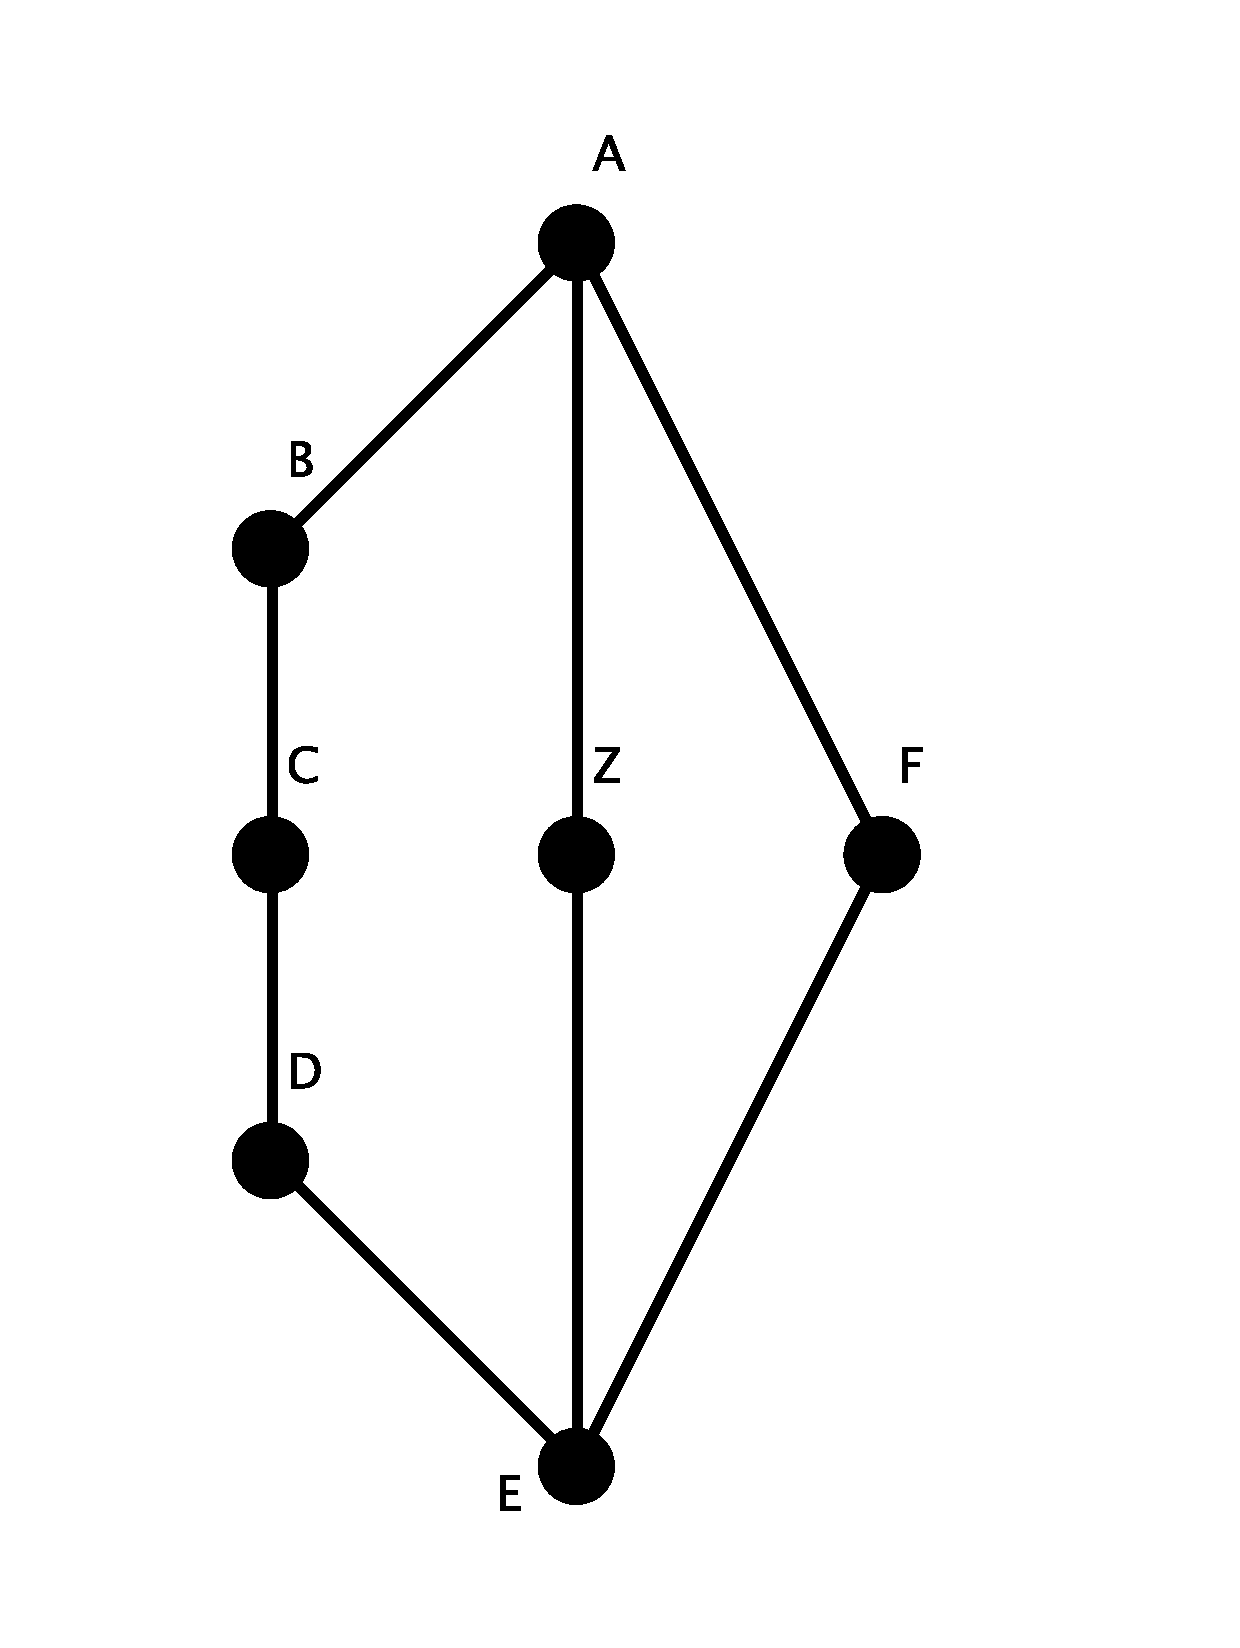
\includegraphics[width=7cm]{obrazky/siblings.pdf}
  \caption{Sourozenci konceptu $Z$}
  \label{fig.siblings}
\end{figure}

V této části popíšeme, jak vygenerovat dotazy, které jsou podobné současnému dotazu, který uživatel zadal do vyhledávače. Když jsme hledali konkrétnější dotazy, hledali jsme je v dolních sousedech; obecnější dotazy jsme hledali v horních sousedech. Podobné dotazy budeme hledat v konceptech, které se nachází na stejné úrovni. Můžeme tak říci, že je budeme hledat v sourozencích konceptu dotazu. 

Otázkou je, jak definovat sourozence. Když se podíváme na obrázek \ref{fig.siblings}, jaké koncepty by měly být sourozenci konceptu $Z$? Když se budeme držet terminologie, která je běžná u binárních stromů, pak by sourozenci byli potomci rodiče, což by odpovídalo sourozencům $\adds{B, F}$. 

U svazů ale můžeme zvolit i opačnou cestu -- rodičové potomků. To by odpovídalo sourozencům $\adds{D, F}$. Dále můžeme říci, že sourozenci jsou všichni mezi potomky a rodiči, tj. všechny koncepty mezi konceptem $A$ a $E$, tj. $\adds{B, C, D, F}$. 

Další rozumnou možností je vzít ty koncepty, které mají stejného rodiče jako koncept $Z$ a zároveň i stejného potomka. Tomu odpovídá koncept $F$.

Pro jednu z těchto definic bychom se měli rozhodnout. Není vhodné uživateli napovídat všechny dotazy z konceptů $B, C$ a $D$, protože $D$ je konkrétnější dotaz než $C$ a $C$ je konkrétnější dotaz než $B$. Z této řady stačí uživateli navrhnout jeden dotaz. 

Pokud budeme za sourozence brát potomky rodičů, budeme mu nabízet spíše obecnější dotazy. Pokud zvolíme rodiče potomků, pak mu budeme nabízet spíše konkrétnější dotazy. 

Zvolíme tak zlatou střední cestu -- budeme mu nabízet dotazy, které generují koncepty, které mají společného rodiče i potomka. Zadefinujeme si funkce, které spočítají všechny horní a dolní sousedy všem prvkům množiny.

\begin{eqnarray}
\unfca(X)&=&\bigcup\adds{\upperneighbors(C)\sep C\in X}\\
\lnfca(X)&=&\bigcup\adds{\lowerneighbors(C)\sep C\in X}
\end{eqnarray}

Nyní můžeme sourozence $\sibl$ konceptu $\hledany$ zadefinovat jako
$$
\sibl_\hledany = \addh{\lnfca(\unfca(\adds{\hledany}))\cap\unfca(\lnfca(\adds{\hledany}))}\setminus\adds{\hledany}.
$$

Z této množiny už jen vytáhneme intenty a dostaneme množinu podobných dotazů
$$
Sibl=\intfca(\sibl_\hledany).
$$

Tyto dotazy setřídíme tak, že spočítáme podobnost konceptů z množiny $\sibl_\hledany$ s konceptem dotazu. Podobnost dvou konceptů spočítáme přes podobnost jejich extentů a intentů. Podobnost dvou extentů pak jednoduše definujeme jako podíl počtu společných objektů a počtu všech objektů. Podobnost dvou konceptů $\addsp{A, B}$ a $\addsp{C, D}$ je rovna
$$
\simfca(\addsp{A, B}, \addsp{C, D}) = \frac12\addk{\frac{|A\cap C|}{|A\cup C|} + \frac{|B\cap D|}{|B\cup D|}}.
$$

Návrh $s_1\in Sibl$ je relevantnější než $s_2\in Sibl$, zapíšeme $s_1\ge s_2$, právě tehdy, když pro koncepty $\addsp{A_1, B_1}, \addsp{A_2, B_2} \in \sibl_\hledany$, jejichž intenty generují $s_1$ a $s_2$, platí $\simfca(\addsp{A_1, B_1}, \hledany)\ge\simfca(\addsp{A_2, B_2}, \hledany)$. Jako první budeme zobrazovat dotaz, který je nejvíce podobný současnému dotazu $Q$.

Téma sousedních konceptů a jejich podobnosti je blíže rozebráno v článku \cite{searchsleuth} a \cite{fcasim}.









%%%%%%%%%%%%%%%%%%%%%%%%%%%%%%%%%%%%%%%%%%%%%%%%%%%%%%%%%%%%%%
%%%%%%%%%%%%%%%%%%%% VÝSLEDKY VYHLEDÁVAČE %%%%%%%%%%%%%%%%%%%%
%%%%%%%%%%%%%%%%%%%%%%%%%%%%%%%%%%%%%%%%%%%%%%%%%%%%%%%%%%%%%%
\newpage
\section{Výsledky vyhledávače}

\ssection{Uživatelské prostředí vyhledávače}
Současná verze vyhledávače \name{} beží na adrese \nameurl. Základní prázdné rozhraní je vidět na obrázku \ref{fig.gui.empty} Do textové pole se vloží dotaz, který chceme položit vyhledávači, vybereme jazyk, databázi, nad kterou chceme dotaz provádět a odešleme. Výsledek vyhledávání je vidět na obrázku \ref{fig.gui.result1}

Na prvních třech řádcích jsou zobrazeny návrhy na úpravu dotazu. Na prvním řádku jsou specializace, tj. jaká slova nabízíme uživateli k přidání k současnému dotazu. Na druhém řádku jsou podobné dotazy. Na třetím řádku je generalizace, tj. jaká slova by měl z dotazu odstranit. Tyto návrhy jsou odkazy, takže na ně stačí klepnout a \name{} vyhledá nový dotaz. 

Níže se nachází část s výsledky vyhledávání a před nimi ještě nějaké informace o dotazu. Na prvním řádku je vypsán celkový počet nalezených dotazů a čas, který byl potřebný na jejich nalezení. Měří to čistě jen práci vyhledávače, jádra, větší množství času je obvykle ztraceno samotnou komunikací mezi jednotlivými vrstvami. 

O řádek níže jsou informace o kontextu a konceptuálním svazu. První dvě položky jsou počty objektů a atributů, které obsahuje kontext, počet dolních a horních sousedů konceptu dotazu a počet jeho sourozenců. Na konci jsou odkazy na zobrazení části svazu, se kterým pracujeme, a na samotný kontext.

\begin{figure}
  \centering
  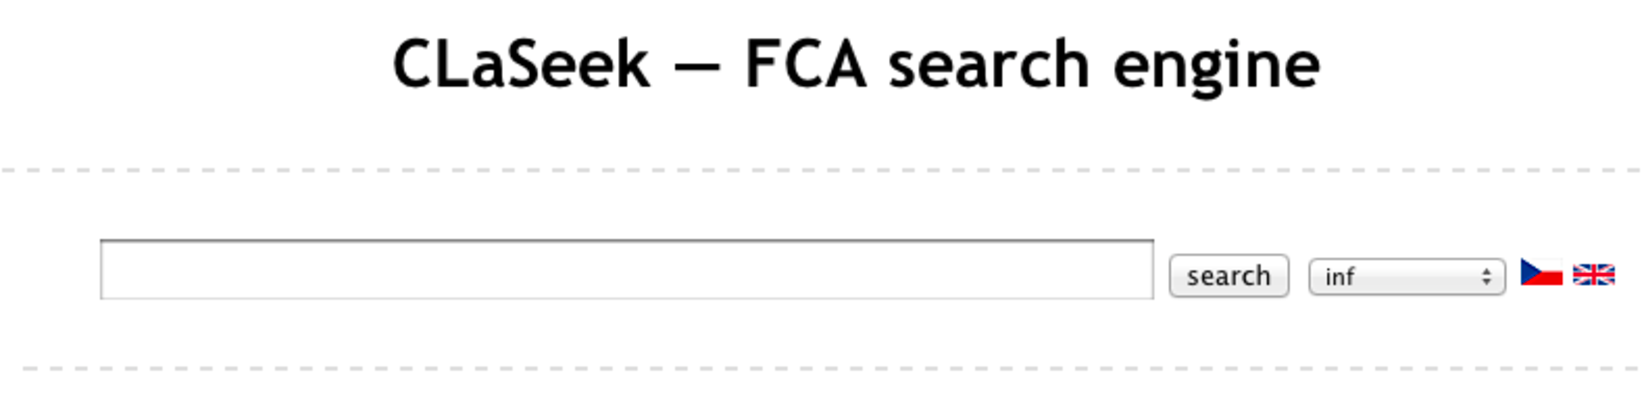
\includegraphics[width=14cm]{obrazky/gui-zakladni.pdf}
  \caption{Základní rozhraní vyhledávače}
  \label{fig.gui.empty}
\end{figure}

\begin{figure}
  \centering
  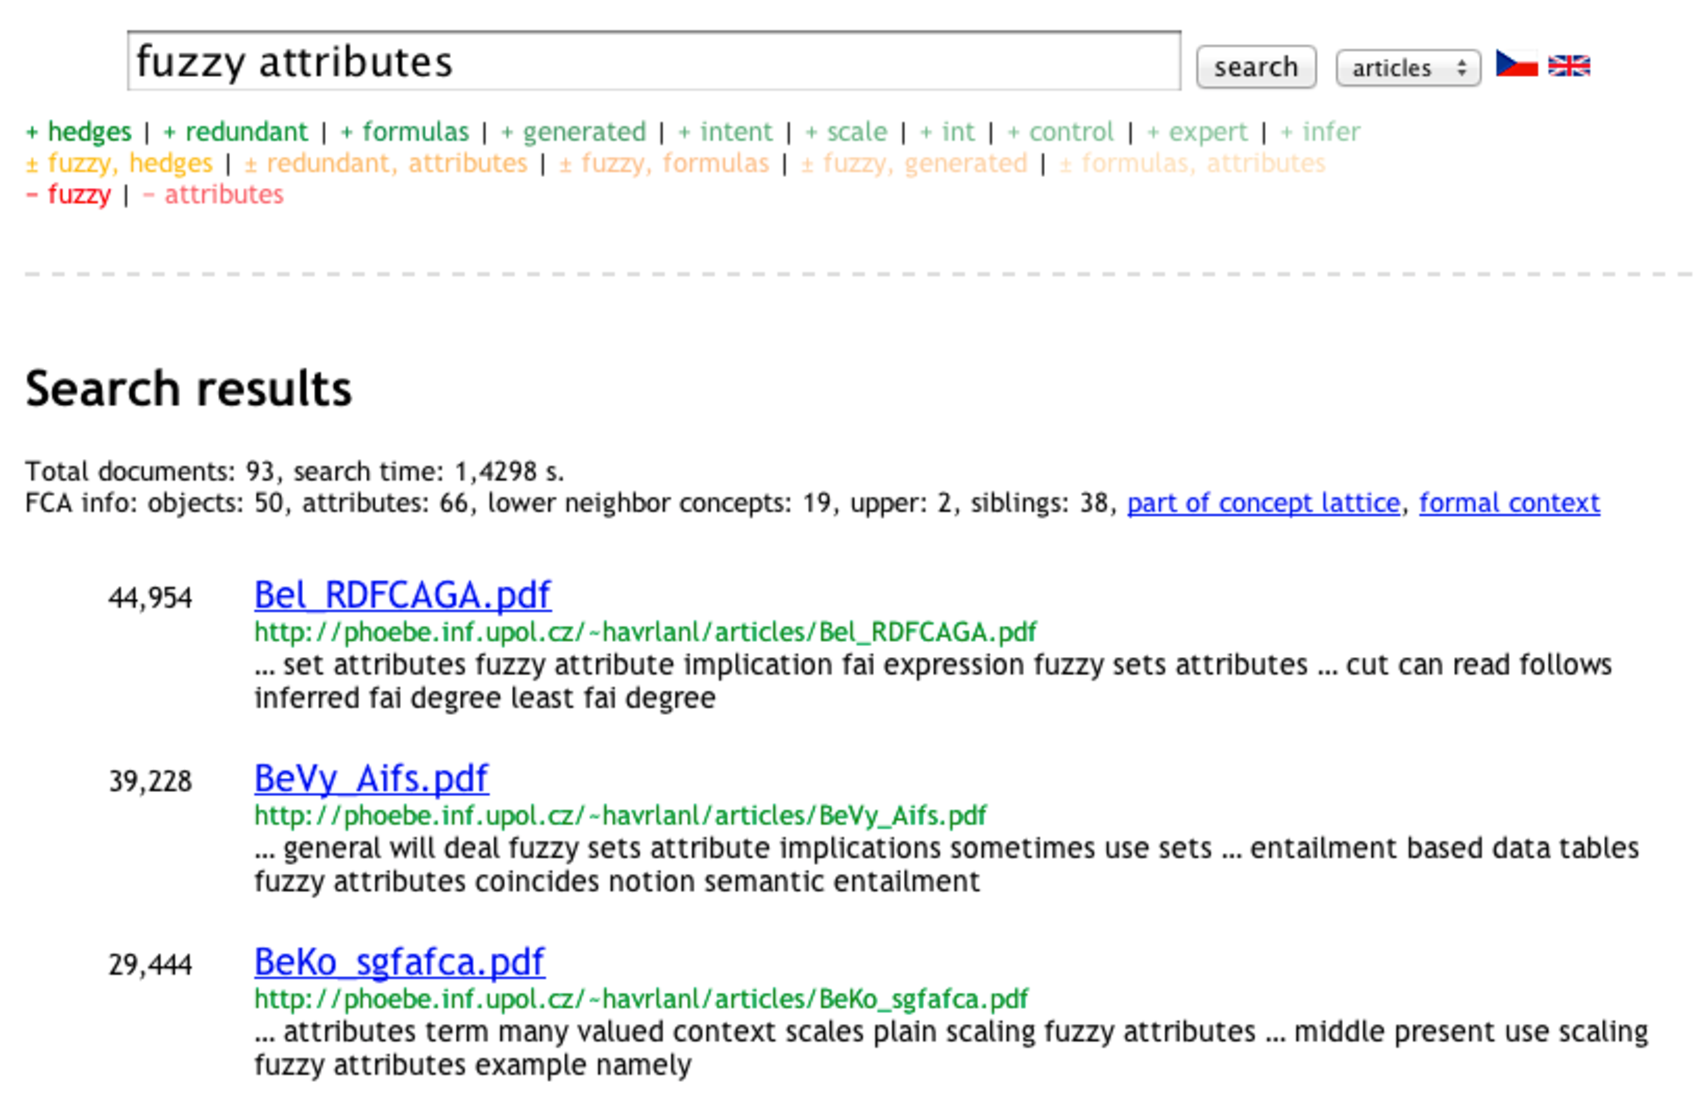
\includegraphics[width=14cm]{obrazky/gui-result1.pdf}
  \caption{Výsledek vyhledávače na dotaz \uv{fuzzy attributes}}
  \label{fig.gui.result1}
\end{figure}

Pak už následují samotné výsledné dokumenty seřazené dle relevance. Vypočítaná hodnota $\tfidf$ pro každý dokument je zobrazena nalevo od odkazů na dokumenty. U dokumentů je nejdříve zobrazen jejich název, pak URL a nakonec popisek. 

\ssection{Požadavky na zpracovávané dokumenty}
Kvalita výsledků v prvé řadě závisí na kvalitě zpracovávaných dokumentů. V této části budou popsány některé vlastnosti, které by dokumenty měly mít, aby \name{} dobře fungoval. 

\sssection{Kvalita obsahů dokumentů}\label{ch.kvalita}
Zásadním požadavkem na dokument je, aby měl dobrý obsah, ze kterého půjde snadno pomocí $\tfidf$ algoritmu získat jeho atributy. Každý dokument by měl mít ideálně jedno hlavní téma a v jeho obsahu by se měla často vyskytovat slova, která toto téma charakterizují. 

Pokud má vyhledávač dobře fungovat, nemělo by se stávat, že stránka \uv{studijní obory} obsahuje pouze seznam studijních oborů, ale samotná slova \uv{studijní} a \uv{obor} se tam nevyskytují buď vůbec, nebo jen v titulku. Vyhledávač se pak nemá čeho chytit, na dotaz \uv{studijní obory} tuto stránku zobrazí někde ke konci seznamu a jako atribut dokumentu zvolí nějaké nesmyslné slovo, které se tam objevuje poměrně často. 

Například pro stránku o studijních oborech na \code{www.inf.upol.cz} zvolil vyhledávač jako hlavní atribut slovo \uv{stupeň}, protože jednotlivé obory jsou tam rozděleny podle stupňů -- 1. stupeň, 2. stupeň, 3. stupeň. Pro prezenční a kombinované studium zvlášť. Samozřejmě zůstává otázkou, jestli by zvýšený počet slov \uv{obor} pomohl i uživateli. 

Vyhledávač si zároveň neumí efektivně poradit se stránkami, které obsahují příliš mnoho různých informací. Na webu katedry informatiky je například takovou stránkou kalendář nebo aktuality. Na těchto stránkách se vyskytují prakticky všechna důležitá klíčová slova. Nachází se zde informace o stážích jednotlivých zaměstnanců katedry, o pořádaných seminářích, informace o oborech a podobně. Každá zpráva v aktualitách nebo v kalendáři je obvykle krátká a podepsaná. 

Když pak uživatel vyhledá jméno nějakého zaměstnance z katedry, často se mezi prvními výsledky zobrazí právě aktuality nebo kalendář, protože samotná stránka není příliš velká, aby to srazilo hodnocení $\tfidf$ a obvykle dané jméno obsahuje mockrát. Podobný výsledek se objeví, pokud vyhledáme slovo \uv{seminář}. Pokud se seminář koná dvacetkrát do roka, má v kalendáři dvacet různých záznamů a kalendář tak obsahuje minimálně dvacetkrát slovo \uv{seminář}. V hodnocení pak snadno předběhne stránku, která je pro informatický seminář přímo určena. Tyto problémy lze vyřešit různými způsoby:

\begin{itemize}
	\item Napsat obsah stránky o informatickém semináři tak, aby obsahoval vícekrát slovo \uv{seminář}.
	\item V hodnocení dokumentů zvýšit důležitost titulků nebo URL, které slovo \uv{seminář} obsahují. 
	\item Využít další informace z celého webu, například text odkazů, které na stránku o informatickém semináři vedou. 
	\item Vyjmout stránky kalendáře a aktualit z indexu, aby se ve výsledcích nezobrazovaly vůbec.
\end{itemize}

\sssection{Technické požadavky na HTML stránky}
Přestože \name{} podporuje další typy souborů jako PDF nebo ODT, je především stavěn pro HTML stránky. Aby vyhledávač dobře fungoval, měl by HTML dokument splňovat některá elementární pravidla. 

Vyhledávač potřebuje u každého dokumentu znát jeho název. V případě HTML stránek ho zjišťuje v elementu \code{TITLE}. Tento element je dle specifikace HTML povinný, takže by ho měla obsahovat každá stránka. Nicméně pokud ho neobsahuje nebo je jeho obsah prázdný, tak se použije poslední část URL. 

Obsah titulku by měl být pro každou stranu jiný. Není vhodné, aby mělo více stránek, nebo dokonce celý web, stejný titulek, protože pak je ve výsledcích vyhledávání nepůjde rozlišit jinak než jejich adresou. Toto pravidlo je důležité nejen pro tento vyhledávač, ale i pro běžné vyhledávače jako Google nebo Seznam. Zároveň se připravujeme o možnost zvýšit hodnocení stránky, pokud by klíčové slovo, které uživatel hledal, bylo v titulku. 

Další informací, kterou může z webu získat, je popisek. Ten se zapisuje do elementu \code{<META NAME='description'>}. Jeho obsahem by měl být ne příliš dlouhý text, který popisuje danou stránku. Opět by měl být unikátní pro každou stránku. Pokud stránka neobsahuje popisek, vyhledávač se pokusí z stránky vytáhnout nějaký popisek sám, ale téměř jistě to bude horší výsledek, než ručně psaný popisek pro každou stránku zvlášť. 

Teoreticky by vyhledávač mohl získávat atributy dokumentů z elementu \code{<META NAME=keywords>}, který je k tomu určen. Ale během historie webu byl tento element poměrně hodně zneužívám vkládáním nesmyslných klíčových slov jako \uv{sex, porno, nahá, pamela, anderson}, takže tento element postupně běžné vyhledávače začaly téměř ignorovat a většina běžných webů už ho ani nepoužívá. \name{} ho tak zcela ignoruje. 

HTML kód nemusí být nutně validní, ale musí dodržovat syntaxi jazyka. Nehledí se například na to, jestli element \code{IMG} obsahuje povinný atribut \code{ALT}, ale pokud nebude hodnota atributu správně ukončena uvozovkami, parser si na tom vyláme zuby. Pro převod HTML stránky do obyčejného textu se ve vyhledávači používají dvě funkce -- první používá vestavěný parser, který postupně parsuje stránku a neodpouští tak žádné chyby proti syntaxi jazyka; druhá funkce používá regulární výrazy a je tak benevolentnější, ale její výsledek je zase méně přesný. Druhá funkce se použije až v případě, kdy selže první funkce.

Web musí mít správně určené kódování stránek prostřednictvím elementu \code{<meta http-equiv='content-type'>}. Pokud se tento element nenajde, bude se předpokládat, že web je v kódování \code{utf-8}. 

\sssection{Zpracování PDF a ODT}
\name{} si dále poradí s dokumenty ve formátu PDF a ODT. Formát ODT je pouze zabalené XML, takže daný soubor stačí pouze rozbalit, najít soubor obsahující obsah celého dokumentu a zpracovat XML. To můžeme udělat podobně jako HTML stránky, stačí odstranit všechny XML značky a nechat pouze textové obsahy elementů. 

S PDF už je větší problém. Vyhledávač používá externí aplikace na dolování textu z PDF souboru, ale žádná aplikace si neporadí se všemi PDF soubory. Největším problémem je diakritika, spousta převaděčů nedokázala po převodu na prostý text správně zobrazit diakritiku. V lepším případě převaděč zobrazil místo správného znaku nějaký nesprávný znak, v horším případě písmeno s dikritikou zcela vypustil, případně vypustil i následující písmeno. S takto převedeným textem už se toho moc dělat nedá. 

Některé PDF dokumenty na webu katedry informatiky jsou v nějakém podivném stavu, kdy i nakopírování textu v některém ze známých PDF prohlížečů, například Adobe Reader, nefunguje jak má. Typická chyba je, že po vložení textu do jiné aplikace jsou zcela oddělené háčky a čárky, občas jsou ještě různě náhodně vloženy mezery. Vyhledávač se snaží alespoň o částečnou rekonstrukci textu, ale úplná rekonstrukce je nemožná. 

\sssection{Některé nedostatky vyhledávače}\label{ch.nedostatky}

Podstatný požadavek je, aby se rozumné atributy nevyskytovala na všech stránkách webu. Tento problém může snadno nastat v případě, kdy jsou na všech stránkách webu stejné odkazy v navigaci. Web katedry informatiky (ale i další zkoumané weby) má na všech stránkách stejnou navigaci, takže slova, která jsou v textech těchto odkazů, mají jen mimální šanci na to, že budou zvoleny atributem nějakého dokumentu. 

Během výpočtu $\tfidf$ funkce hledáme taková slova, která se často vyskytují v daném dokumentu, ale co nejméně ve všech ostatních dokumentech. Funkce bohužel nezkoumá, kolikrát se dané slovo v těch ostatních dokumentech nachází, takže stačí, když se v dokumentu nachází jen jednou v navigaci a už se to bude počítat jako výskyt. 

Kódování HTML stránky lze definovat i HTTP hlavičkou. Samotná stránka pak nemusí obsahovat element \code{<meta http-equiv='content-type'>}. Vzhledem k tomu, že \name{} HTTP hlavičky nezkoumá, použil by v tomto případě výchozí kódování \code{utf-8}. 

\ssection{Hodnocení úspěšnosti vyhledávače}
Ohodnotit, jak je \name{} úspěšný v řazení nebo v nabízených návrzích, nijak exaktně a automaticky nejde. Zbývá jen ruční zkoumání a slovní ohodnocení. 

Ve vyhledávači je uloženo několik testovacích sad dokumentů. Jedná se o weby 
\begin{itemize}
	\item \code{jakpsatweb.cz}, který se zabývá tvorbou webových stránek a podobných věcech okolo, 
	\item \code{matweb.cz}, který se zabývá především středoškolskou matematikou,
	\item \code{jakpodnikat.cz}, který se zabývá podnikáním, jak danit příjmy a podobně,
	\item \code{inf.upol.cz}, což je web katedry informatiky UP
\end{itemize}
a nakonec je ve vyhledávači použita i sada volně stažitelných odborných článků ve formátu PDF, které napsali zaměstnanci katedry informatiky UP. 

Kromě webu katedry informatiky se jedná o weby, které mají jasné zaměření každé stránky a bohatý obsah, takže na jejich webech vypadá analýza nejlépe. Web katedry informatiky je stručnější, obsahuje jisté chyby (například titulky pro každou stranu zvlášť, jak je psáno v kapitole \ref{ch.kvalita}, byly vytvořeny až během psaní této práce) a obsahuje nepříjemnost v podobě opakujících se slov na každé stránce, viz kapitolu \ref{ch.nedostatky}, takže jeho analýza neprobíhá nejlépe. 

\sssection{Příklady dobrých výsledků}
Analýza webu jakpodnikat.cz dává několik dobrých výsledků, pro příklad:

\begin{itemize}
	\item Na dotaz \uv{živnostenský list} vrací seznam specializací \code{+ studenti | + příjmy | + provozovna | + nemocenské | + účetnictví | + jednotný | + dědická | + odkazy | + nemovitostí | + auto}.
	\item Když k dotazu přidáme například slovo \uv{provozovna}, vyhledávač odpoví novými specializacemi \code{+ studenti | + příjmy | + zahájení | + služby | + autorský | + nemovitostí}. Zároveň přidá i podobné dotazy \code{+/- list, příjmy, živnostenský | +/- list, zahájení, živnostenský | +/- autorský, list, živnostenský | +/- nemovitostí, list, živnostenský}.
	\item Po vyhledání dotazu \uv{slevy na dani} dostaneme specializace \code{+ příjmy | + studenti | + základ | + doklady | + tisíc | + příloha | + minimální}, z nichž všechny kromě slova \uv{tisíc} dávají nějaký smysl. Seznam podobných dotazů: \code{+/- dani, příjmy | +/- dani, základ | +/- dani, doklady | +/- tisíc, dani | +/- příloha, dani}. Opět kromě dotazu, který obsahuje klíčové slovo \uv{tisíc} to má nějaký smysl. 
\end{itemize}

Dobré výsledky vrací \name{} i pro web jakpsatweb.cz: 

\begin{itemize}
	\item Pro dotaz \uv{hosting} vrátí seznam specializací \code{+ php | + serveru | + seo | + google | + weblogu | + zdarma | + nástroje | + statistiky | + domény | + anglicky}. 
	\item Pokud přidáme slovo \uv{php}, dostaneme nový seznam specializací \code{+ serveru | + knihy | + google | + zdarma | + faq | + díky | + weblogu | + xml | + seo | + statistiky} a seznam podobných dotazů: \code{+/- hosting, serveru | +/- google, hosting | +/- hosting, zdarma | +/- knihy, php | +/- php, zdarma}.
\end{itemize}

\sssection{Příklady špatných výsledků}

Ze současných databází dává většinou nejhorší výsledky web katedry informatiky. Příkladem budiž dotaz \uv{studium}, na který získáme specializace \code{+ zimní | + absolvent | + letní | + skupina | + jan | + martin | + arnošt | + činnosti | + szz | + bartl}. Většina těchto dotazů nejspíše k žádnému významnému konceptu nepovede. 

Dalším příkladem může být složitější dotaz \uv{jak vložit obrázek na stránku} nad databází jakpsatweb.cz. Vyhledávač odpoví specializacemi \code{+ obrázky | + soubor | + google | + mail}. Nabízí to dokonce slovo \uv{obrázky}, protože použitý stemmer zvolí jiný základ pro slovo \uv{obrázek} a pro \uv{obrázky}. Další návrhy nejsou o nic rozumnější. 


\ssection{Experimenty s nastavením}
\name{} umožňuje má poměrně bohaté možnosti nastavení. Některé z nich dokáží významně ovlivnit chování a výsledky celého vyhledávače. Všechny možnosti nastavení jsou popsány v kapitole \ref{ch.dokumentace}

\sssection{Počet atributů dokumentu}
Lze nastavit, jaký maximální počet atributů každého dokumentu vyhledávač vezme v potaz, když buduje rozšířený koncept, viz kapitolu \ref{ch.sestaveni} To do jisté míry ovlivní, jak budou vypadat jednotlivé návrhy u specializací a u podobných dotazů. 

Čím vyšší limit nastavíme, tím větší bude kontext a tím více bude mít koncept dotazu dolních sousedů a sourozenců. Což v důsledku znamená, že vyhledávač má na konci více návrhů na specializaci a více podobných dotazů. Zvyšuje se tím šance, že se v této množině návrhů najde nějaký smysluplný návrh, ale zároveň se zvyšuje šance, že se tam dostane nějaký nesmysl, protože některý dokument nemusí mít tolik kvalitních atributů. 

Brát v úvahu vysoký počet atributů dokumentů má smysl v případě, kdy víme, že k většině dokumentů máme alespoň tolik kvalitních atributů. Pokud není pravděpodobné, že bychom k většině dokumentů nalezli tolik kvalitních atributů, raději snížíme počet atributů, které bereme v potaz. 

Zvýšení počtu atributů má samozřejmě za následek mírně zpomalení celého programu, protože se pracuje s větším kontextem a větším svazem. 

\sssection{Počet dokumentů v kontextu}
V nastavení můžeme omezit počet dokumentů, které budou tvořit množinu objektů rozšířeného kontextu. Výsledek je podobný jako v předchozím případě -- pokud zvýšíme počet dokumentů, které pustíme do kontextu, zvýšíme tím šanci, že se mezi návrhy nějaký zajímavý, který by se tam jinak neobjevil. Současně tím ale zvyšujeme šanci, že se tam objeví nesmysl, protože jsme do kontextu pustili dokumenty, které jsou příliš vzdálené původnímu dotazu.

Zároveň při větším počtu dotazů roste výpočetní náročnost, protože se zvětšuje kontext a konceptuální svaz. Zvyšuje se více než v předchozím případě, protože tím, že zdvojnásobíme počet dokumentů, zdvojnásobí se i počet atributů. 

\sssection{Limit pro atributy dokumentu}
Během budování indexu je možné zvolit dvě hlavní kritéria, jak se budou hledat atributy dokumentů. Jednodušší verze je, že vyhledávač spočítá $\tfidf$ skóre pro všechna slova v dokumentu a poté vezme $n$ slov, která mají toto skóre nejvyšší. Druhý způsob je, že vezmeme jen ta slova, která překročila určitou hranici skóre. 

První způsob je přímočarý, ale není příliš efektivní v případě, kdy máme různě kvalitní dokumenty. Pro ty nekvalitní dokumenty, u kterých lze jen těžko najít tolik smysluplných atributů, se budou za atributy postupně volit čím dál tím větší nesmysly. Výhodou je, že pro každý dokument máme stejný počet atributů.

U druhého způsobu je o něco těžší nalézt ideální hranici. Hranice je číslo z intervalu $\addsp{0, 100}$ a bude aplikována takto: spočítáme hodnotu $\tfidf$ skóre pro všechna slova ve všech dokumentech. Tato čísla seřadíme, dostaneme tak uspořádaný seznam ohodnocených slov. 

Ze začátku a z konce tohoto seznamu odstraníme setinu slov. Pokud seznam obsahuje 500 slov, pak ze začátku i z konce seznamu odstraníme pět slov. Tím odstraníme slova, která by mohla mít příliš vysoké nebo příliš nízké hodnocení. Dále spočítáme rozdíl největšího a nejmenšího hodnocení. Tento rozdíl si označíme $\delta$. Hranici vydělíme stem, abychom získali číslo v intervalu $\addsp{0, 1}$, označme tuto novou hodnotu $l$. Dále ještě označme nejmenší hodnotu skóre ze všech slov symbolem $m$. 

Pak každé slovo, které má hodnotu $\tfidf$ skóre alespoň $l\cdot\delta+m$ bude považováno za atribut daného dokumentu. 










%%%%%%%%%%%%%%%%%%%%%%%%%%%%%%%%%%%%%%%%%%%%%%%%%
%%%%%%%%%%%%%%%%%%%% DODATKY %%%%%%%%%%%%%%%%%%%%
%%%%%%%%%%%%%%%%%%%%%%%%%%%%%%%%%%%%%%%%%%%%%%%%%

\newpage
\section{Dodatky}

\ssection{API vyhledávače}

API aplikace je rozhraní, pomocí něhož může uživatel s danou aplikací komunikovat. Uživatel aplikaci posílá nějaké dotazy ve specifickém formátu a aplikace na ně opět ve specifickém formátu odpovídá. Uživatel tak může danou aplikaci používat, ačkoliv ji přímo nezkompiluje do své aplikace.  

Jak jádro vyhledávače, tak webové rozhraní poskytuje API pro uživatele. Webové API je přístupné komukoliv, konzolové API je přístupné tomu, kdo si nainstaluje vyhledávač k sobě. Webové API je RESTové, to znamená, že využívá HTTP protokol a běžné metody jako GET nebo POST. Všechna data, která vyhledávač vrací na výstupu, jsou ve formátu JSON. Pro detaily viz kapitolu \ref{ch.dokumentace}

\sssection{Získávání dat z indexu}

\name{} umožňuje získávat data o existujících indexech. Ta se získávají pomocí HTTP GET požadavku s požadovanými parametry. Je možné zjistit například informace o daném dokumentu, jaký má titulek, jakou adresu a podobně. Zároveň lze zjisit další informace o indexu, například počet všech zaindexovaných dokumentů nebo seznam URL adres všech dokumentů.

Například dotazem \code{/api.php?d=jpw\&docinfo=147\&title} zjistíme název dokumentu z databáze \code{jpw}, který má ID 147.

\sssection{Posílání vlastních dat na server}\label{ch.apipost}
API vyhledávače umožňuje poslat na server vlastní dokumenty a provést nad nimi FCA analýzu. To se děje HTTP POST požadavkem. Poslaná data musí být ve formátu JSON. \name{} tyto dokumenty přijme, zpracuje je, tj. provede úplně stejné operace, jako by budoval klasický index, vytvoří dočasný index a následně nad těmito daty provede standardní FCA analýzu, jaká byla popsána v předchozích částech dokumentu. 

Výsledkem budou opět data ve formátu JSON, která budou obsahovat výsledek FCA analýzy. Nalezneme tam specializace, generalizace a podobné dotazy a některá další data o kontextu a konceptuálním svazu. Dále tam bude seznam dokumentů, který bude seřazený dle relevance. Výstup je prakticky stejný, jako je grafický výstup vyhledávače, pouze máme výsledky v surové JSON podobě. 

Tohoto můžeme využít na vylepšení výsledků běžného vyhledávače, například Googlu. Napíšeme webovou aplikaci, na které bude textové pole pro zadání dotazu. Uživatel zadá dotaz, aplikace tento dotaz přepošle API Googlu a získá výsledky pro zadaný dotaz. Následně převede výsledky z Googlu do takového formátu, kterému rozumí vyhledávač.

My od Google získáme seznam několika odkazů, které odpovídají zadanému dotazu. Pro každý odkaz máme k dispozici tři zásadní údaje: URL, titulek a popisek. Z těchto tří údajů vytvoříme sadu dokumentů takto: každý odkaz bude tvořit jeden samostatný dokument. Takže pokud nám Google vrátí na dotaz 50 výsledků, budeme vytvářet 50 dokumentů. URL dokumentu bude stejné jako URL, které vrátil Google; stejně tak titulek. Obsahem dokumentu pak bude popisek odkazu. Popisek dokumentu může být buď stejný jako jeho obsah nebo bude prázdný.

Takto poskládaná data, zároveň s původním dotazem, který jsme kladli Googlu, pošleme vyhledávači. On z nich seskládá dočasný index a vrátí nám návrhy, které vygenerovala FCA analýza. Tyto návrhy pak můžeme předložit uživateli. Tím dostaneme aplikaci, která už téměř stejná jako SearchSleuth.

Jednou z cest, kam může směřovat tento vyhledávač, je rozšíření API a napsání dalších aplikací, které toto API využívají. Jednoduchou úpravou algoritmů ve vyhledávači můžeme například vytvořit API, které bere na vstupu seznam dokumentů a na výstupu vrací kategorizovaný seznam dokumentů -- ke každému dokumentu přiřadí jednu, případně i více, kategorii. To se může hodit v případě, kdy máme velké množství dokumentů, které chceme setřídit do nějakých kategorií. Podobných způsobů využití lze jistě vymyslet více. 


\ssection{Struktura aplikace a používané programy}
Jádro vyhledávače je psáno v Pythonu 3, nainstalovaná verze pak běží na Pythonu 3.2. Zdrojové soubory jsou rozděleny do balíčků, které obsahují moduly. Mezi nejdůležitější balíčky patří: 

\begin{description}
	\item[\code{preprocess}:] Obsahuje moduly, které jsou zodpovědné za budování nového indexu, úpravu existujícího indexu, odstranění HTML značek z HTML stránek a podobně. 
	\item[\code{retrieval}:] Tento balíček je zodpovědný za dolování informací z indexu, parsování dotazu nebo hodnocení dokumentů. 
	\item[\code{fca}:] Definuje základní struktury pro práci s FCA, jako například kontext nebo koncept. 
	\item[\code{fca-extension}:] Po získání dat z indexu se moduly z tohoto balíčku snaží nalézt správné návrhy na vylepšení dotazu. 
\end{description}

Veškerou komunikaci s externími aplikacemi pak obstarává soubor \code{/src/search}, který volá funkce z modulu \code{/src/other/interface.py}. Ten obsahuje funkce zodpovědné za komunikaci se všemi ostatními balíčky a moduly. 

Aplikace používá dva stemmery, jeden pro český jazyk a jeden pro anglický. Pro český jazyk je využit kód, který napsal Ljiljana Dolamic, jako anglický stemmer je použit program implementující Porter2 algoritmus a jehož autorem je Matt Chaput. Pro převod PDF do prostého textu aplikace používá program Xpdf \url{http://www.foolabs.com/xpdf/}. Na převod ODT do prostého textu není použita žádná externí aplikace, pouze \code{unzip} a obecný XML parser. 

Webové rozhraní je napsáno v PHP 5. HTML kód je validní dle současného návrhu HTML 5. 

\ssection{Dokumentace}\label{ch.dokumentace}
Dokumentace k jednotlivým částem programu se nachází na webu spolu se zdrojovými kódy aplikací. K distribuci zdrojového kódu byl použit web \code{www.github.com}, přesné adresy jednotlivých projektů: 

Zdrojové kódy jádra vyhledávače se nachází na adrese
\begin{itemize}
	\item \code{https://github.com/havrlant/fca-search}
\end{itemize}
Dokumentace, popis všech možností nastavení a popis API jádra aplikace se nachází na wiki stránce
\begin{itemize}
	\item \code{https://github.com/havrlant/fca-search/wiki/dokumentace}
\end{itemize}
Zdrojové kódy webového rozhraní se nachází na adrese
\begin{itemize}
	\item \code{https://github.com/havrlant/fca-seach-web}
\end{itemize}
Dokumentace, popis všech možností nastavení a popis API webového rozhraní se nachází na wiki stránce
\begin{itemize}
	\item \code{https://github.com/havrlant/fca-seach-web/wiki/dokumentace}
\end{itemize}
Zdrojového kódy ukázky práce s API se nachází na adrese:
\begin{itemize}
	\item \code{https://github.com/havrlant/fca-seach-api-test}
\end{itemize}
Zdrojové kódy tohoto textu se nachází na adrese:
\begin{itemize}
	\item \code{https://github.com/havrlant/fca-search-text}
\end{itemize}

\ssection{Podobné vyhledávače}\label{ch.fcaengines}
V historii již existovaly vyhledávače, které fungovaly velice podobně jako \name. Jedná se o vyhledávače \uv{CREDO}, \uv{FooCA} a \uv{SearchSleuth}. V současné době CREDO a SearchSleuth nefungují vůbec a k použití FooCA je nutné zažádat o registraci tvůrce tohoto vyhledávače. 

\begin{description}
	\item[CREDO] Zkratka pochází z \uv{Conceptual REorganization of DOcuments}. Jeho autory jsou C. Carpineto a G. Romano. CREDO spolupracovalo s Googlem, vložený dotaz nejprve vložile pomocí do Google SOAP API, nechalo si vrátit prvních 100 výsledků a poté nad těmito daty provedlo FCA analýzu. CREDO počítalo pouze dolní sousedy a to do druhé úrovně. Začínalo se u největšího konceptu. Smyslem bylo, abych z těch sto výsledků, které dostal na začátku, postupně ukazoval uživateli ty odkazy, které odpovídají nějakému konceptu. 

	CREDO poté zobrazilo uživateli seznam odkazů spolu se stromovou strukturou návrhů na změnu dotazu. Tyto návrhy ale nebyly interaktivní, pouze, po kliknutí na návrh, se z té stovky vrácených dotazů vyfiltrovaly ty, které odpovídaly novému dotazu. Žádný nový dotaz do Google neproběhl. Detailnější informace jsou v článku \cite{credo}.

	\item[FooCA] Název vznikl ze spojení FCA a Google. Autorem je Bjoern Koester. Vyhledávač funguje na adrese \code{http://fooca.webstrategy.de}, ale vyžaduje registraci. FooCA, podobně jako CREDO, spolupracuje s webovými vyhledávači, konkrétně s Googlem a Yahoo. Uživatel vloží dotaz do Foo\-CA, ten přepošle dotaz beze změny do Google API nebo do Yahoo API a dále pracuje s navrácenými výsledky. Po skončení FCA analýzy zobrazí uživateli výsledek ve formě tabulky -- kontextu -- nebo ve formě diagramu znázorňující konceptuální svaz. 

	Detailnější informace jsou v článku \cite{fooca}.
	\item[SearchSleuth] je nejvíce podobný vyhledávači popsanému v této práci. Jeho autory jsou J. Ducrou a P. Eklund. SearchSleuth  spolupracoval s Yahoo a jeho API. Po obdržení výsledků od vyhledávače sestaví kontext, nalezne koncept dotazu a znovu vyhledá ve vyhledávači obsah intentů horních sousedů, čímž SearchSleuth získá více výsledků a může sestavit rozšířený kontext. \name{} toto provádí pomocí dodatečného OR dotazu. SearchSleuth také do kontextu nepřidává klíčová slova z dotazu. Jinak je FCA část obou vyhledávačů velice podobná. 

	Detailnější informace jsou v článku \cite{searchsleuth} a \cite{fcasim}. Podobný systém byl také použit například pro analýzu CHM souborů, proprietárního formátu Microsoftu pro nápovědu. Více informací v \cite{helpsleuth}.
\end{description} 





%%% Závěr práce v~češtině
\begin{conclusions-cz}

Výsledkem této práce je prototyp webového vyhledávače \name{}, který primárně pracuje nad statickou sadou dokumentů. Umí prohledávat několik typů dokumentů, automaticky z dokumentů získávat název a popisek, zvládá booleovské dotazy, kontroluje překlepy a výsledné dokumenty vrací seřazené dle relevance. 

Po navrácení výsledných dokumentů provádí jejich analýzu a prostřednictvím formální konceptuální analýzy nabízí tři skupiny návrhů na úpravu dotazu. Konkrétnější dotazy, obecnější dotazy a podobné dotazy. \name{} tak pomáhá uživateli upravovat dotaz tak dlouho, dokud není spokojen s výsledky vyhledávání. 

\name{} dále poskytuje veřejné webové API, díky kterému je možné vyhledávači zasílat vlastní data. Vyhledávač pak sestaví dočasný index a provede nad zaslanými daty stejnou analýzu, jako v případě statického indexu. 

Kvalita výsledků je přímo úměrná kvalitě zaindexovaných dokumentů. Pokud do vyhledávače vložíme obsahově bohaté dokumenty, jsou návrhy většinou dobré. Celá analýza je poměrně rychlá, \name{} pro daný dotaz vrátí všechny výsledky obvykle za několik sekund. Všechny kódy jsou volně přístupné pod BSD licencí a vyhledávač tak lze případně nainstalovat na vlastní server. 

Další výzkum může proběhnout v části, která zpracovává samotné dokumenty. Například vylepšit algoritmy, které hledají atributy dokumentů, zdokonalit stemmer, zjišťovat synonyma a podobně. V části hledající návrhy je možné zavést fuzzy FCA, kdy do formálního kontextu neuložíme pouze informace o tom, zda dokument dané slovo obsahuje, ale i informaci o tom, jak moc je slovo pro dokument důležité. Je možné také rozšířit API, které \name{} nabízí a nad tímto API postavit další externí služby. 
\end{conclusions-cz}


%%% Závěr práce v~angličtině
\begin{conclusions-en}
\name{} is a prototype of a web search engine that works with static set of documents. It can process several types of documents, extracts a title and a description of a document, handles Boolean queries, checks typing errors and the result set of documents is ordered by relevance.

After retrieving the result set of documents, formal concept analysis is performed. We try to find three types of query suggestions: generalisations, specialisations and categorisation. \name{} helps user to refine query until he is satisfied with the result. 

\name{} provides a public web API. It can be used to post your own data. The search engine builds up a temporary index and then formal concept analysis is performed to obtain query suggestions. 

The quality of results is determined by the quality of the documents. If we put into the search engine documents with rich and good content we usually obtain good results. The analysis is rather quick. \name{} returns results for a single query in a few seconds. The search engine is open source software under the BSD licence so everyone can use it on their own server. 

Further research can be done in the following areas: document processing like improve attributes searching, improve stemmer, search for synonyms, etc. We can use fuzzy FCA instead of crisp FCA. We can use information about word importance to build a new fuzzy formal context. We can extend API and create some new applications that use it. 
\end{conclusions-en}

\newpage
% Diplomka používá Český styl pro BibTex, jehož autorem je David Martinek
% Zdroj: http://www.fit.vutbr.cz/~martinek/latex/czechiso.html
\bibliographystyle{czechiso}
\bibliography{citace}

\newpage
\appendix

\section{Obsah přiloženého CD}
Popis struktury přiloženého CD:

\begin{description}
	\item[bin] 
	\item[doc]
	\item[]
\end{description}

\end{document}